\chapter{Introduzione}

\section{Modello Standard}

{\bf MA TUTTO QUESTO PIPPONE SUL MS SERVE??????}

Il {\em Modello Standard} (MS) è la teoria che ad oggi descrive meglio la fenomenologia delle interazioni tra particelle elementari. Questa teoria, formulata nella seconda metà del novecento riesce a descrivere tre delle quattro interazioni fondamentali: interazione elettromagnetica, interazione debole e interazione forte, mentre ad oggi non esiste una estensione della teoria che comprenda l'interazione gravitazionale.

\begin{figure}
\centering
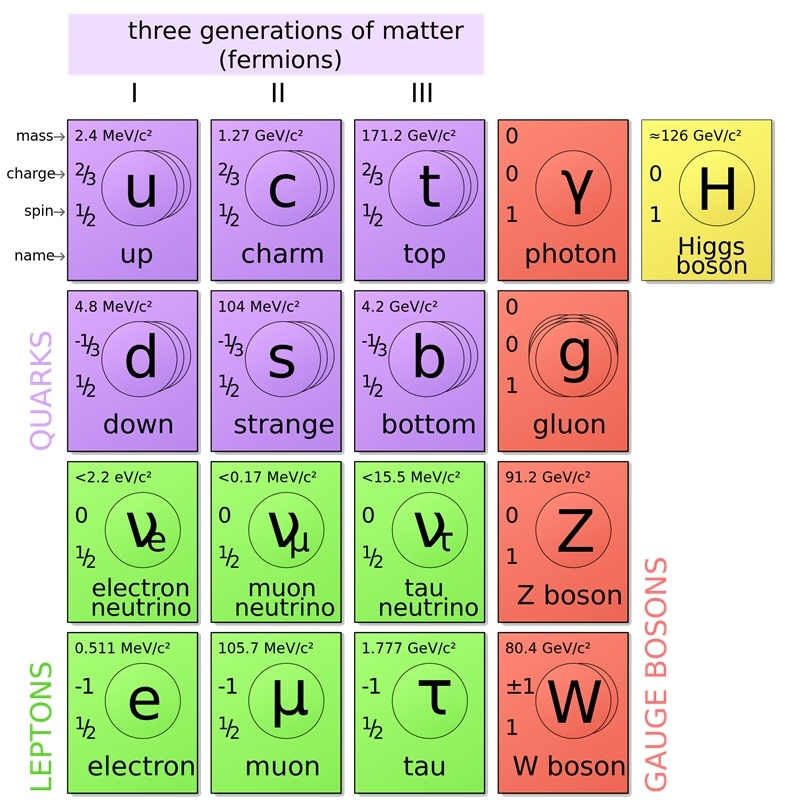
\includegraphics[scale=0.3]{Immagini/SM}
\caption{Particelle elementari del Modello Standard.}
\label{fig:SM}
\end{figure}

Il Modello Standard descrive la materia come composta da due tipi di particelle, entrambi fermioni con spin $\nicefrac{1}{2}$, {\em leptoni} e {\em quark}:

\begin{itemize}
\item i {\em leptoni} hanno carica elettrica intera e quelli conosciuti sono sei, suddivisi in tre generazioni di doppietti con massa crescente. Ogni doppietto è costituito da una particella con carica $Q=-1$ che ha interazioni elettrodeboli, rispettivamente l'elettrone $e$, il muone $\mu$ e il leptone tau $\tau$ nelle tre generazioni. Il doppietto \`e completato da una particella neutra chiamata {\em neutrino}, $\nu_e$, $\nu_{\mu}$ e $\nu_{\tau}$ rispettivamente, che interagisce solo per interazione debole.
\item Analogamente ai leptoni i {\em quark} sono organizzati in doppietti. In questo caso però la carica è frazionaria: la componente superiore del doppietto ha carica $Q=2/3$ ed \`e costituita dai quark $u$, $c$ e $t$ rispettivamente per le tre generazioni. La componente inferiore ha carica $Q=-1/3$ ed \`e costituita dai quark $d$, $s$ e $b$ rispettivamente per le tre generazioni. I quark interagiscono sia elettrodebole che forte e quest'ultima interazione è alla base della formazione di stati legati chiamati adroni, come ad esempio neutrone e protone.
\end{itemize}

Ad ognuna di queste particelle corrisponde una antiparticella che ha i numeri quantici opposti ma stessa massa e spin. Oltre alle antiparticelle il Modello Standard prevede l'esistenza dei {\em bosoni di gauge} e del {\em bosone di Higgs}. I primi sono i mediatori delle interazioni che, a loro volta, derivano dalle simmetrie insite nella teoria:

\begin{itemize}
\item il {\em fotone} \`e responsabile della mediazione dell'interazione elettromagnetica;
\item i {\em bosoni $W^{\pm}$} e $Z$, sono i mediatori dell'interazione debole; un'esempio in cui entra in gioco questa forza è il decadimento $\beta$. Questi bosoni, sono massivi, circa $80\GeVcc$ e $91\GeVcc$ rispettivamente.
\item I {\em gluoni} sono i mediatori dell'interazione forte.
\end{itemize}

Come detto precedentemente la forza gravitazionale non è descritta dal MS, ma risulta essere trascurabile nelle interazione tra particelle, in quanto la sua intensità, paragonata a quella delle altre tre forze, è vari ordini di grandezza inferiore. Nel MS le interazioni sono descritte come manifestazioni di simmetrie di gauge della Lagrangiana. Queste simmetrie non ammettono termini di massa per i bosoni di gauge poiché questo porterebbe alla rottura delle simmetrie stesse. Tuttavia \`e possibile introdurre un meccanismo di rottura spontanea della simmetria, detto {\em di Higgs}, da cui derivano i termini di massa per i bosoni di gauge e un ulteriore bosone scalare massivo, il {\em bosone di Higgs} H. Attraverso il meccanismo di Higgs vengono anche introdotti i termini di massa dei fermioni.

{\bf Aggiungere un paragrafetto sulle problematiche del MS (dark matter, teoria efficace a bassa energia etc.). Per questo si costruiscono gli acceleratori ...}

\section{LHC e l'esperimento CMS}
Il {\em Large Hadron Collider} o {\em LHC} è attualmente il più grande acceleratore di particelle mai costruito. Si trova presso il {\em CERN} ({\em European Organization for Nuclear Research}), collocato in un anello sotterraneo di 27~km nella regione di Ginevra (Svizzera). 

LHC \`e un collider adronico in grado di produrre interazioni protone-protone all'energia di $13\TeV$ nel centro di massa. \`E stato progettato con due anelli separati con campo magnetico opposto in modo che i fasci controrotanti possano essere costituiti da particelle con la stessa carica elettrica. Questa caratteristica, oltre ad altre, fa di LHC una macchina di frontiera di ineguagliata complessit\`a che ha richiesto una grande innovazione tecnologica. 

L'accelerazione dei protoni avviene a stadi come schematizzato in~Fig.~\ref{fig:LHC}: i protoni ottenuti da idrogeno gassoso sono inizialmente accelerati da un acceleratore lineare, LINAC2. Successvamente i protoni sono iniettati nel Proton Synchroton Booster (PSB) che aumenta l'energia fino a $1.4\GeV$ e, in seguito, grazie al Proton Synchrotron, raggiungono i $25\GeV$. In queste fasi i protoni vengono raggruppati in pacchetti distanti temporalmente $25\ns$ intervallo che che corrisponde alla frequenza di interazioni di $40\MHz$ a cui LHC opera. 
I protoni vengono infine accelerati fino ad energie di $450\GeV$ nel Super Proton Synchrotron (SPS) prima di essere iniettati nei due anelli di LHC in cui subiscono l'ultima fase di accelerazione fino all'energia di $13\TeV$ prima di farli collidere nei punti in cui sono collocati gli esperimenti.

Il {\em Compact Muon Solenoid} o {\em CMS} è uno dei principali esperimenti di LHC, assieme ad ALICE, ATLAS e LHCb. 

\begin{figure}
\centering
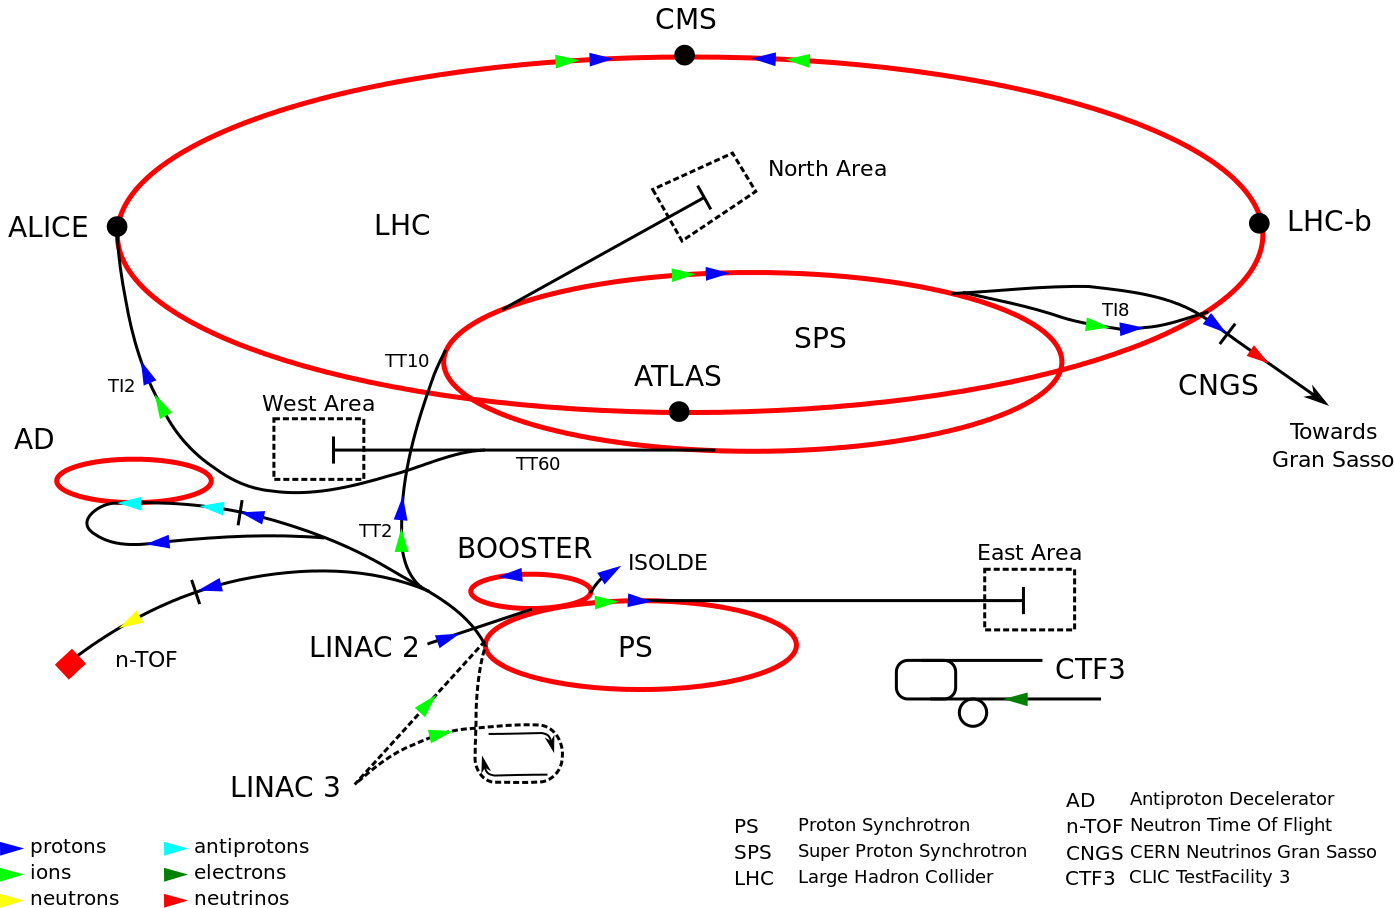
\includegraphics[scale=0.25]{Immagini/LHC}
\caption{Schema di pre-accelerazione e accelerazione di LHC.}
\label{fig:LHC}
\end{figure}

Lo scopo di questi esperimenti è lo studio del MS e la ricerca della materia oscura e di evidenze di nuova fisica, ovvero fenomeni non previsti dal MS stesso. Questi esperimenti sono collocati nei punti in cui i fasci di particelle si incrociano e le interazioni protone-protone prodotte possono essere quindi registrate ed essere analizzate in seguito. Pi\`u nel dettaglio:
\begin{itemize}
\item ALICE (A Large Ion Collider Experiment) \`e un esperimento che studia un stato della materia noto come {\em quark-gluon plasma}, prodotto nelle collisioni di ioni pesanti dal momento che, oltre alle collisioni protone-protone, LHC pu\`o operare come collisionatore ione-ione;
\item CMS (Compact Muon Solenoid) e ATLAS (A Toroidal LHC ApparatuS) sono entrambi progettati con lo scopo di investigare il più ampio spettro di fisica possibile. I due esperimenti hanno gli stessi obbiettivi, ma sono stati costruiti in modo differente al fine di essere indipendenti nello studio dei processi di interazione che avvengono durante le collisioni tra due protoni. Atlas e CMS nel 2012 hanno scoperto il bosone di Higgs~\cite{scopertahiggs}. 
\item LHCb (LHC beauty) \`e un esperimento che studia la fisica degli adroni contenenti il quark b e la violazione di CP (coniugazione di Carica e Parità) nelle interazioni elettrodeboli.
\end{itemize}
Altri esperimenti presenti ad LHC, ma di dimensioni minori sono TOTEM e LHCf:
\begin{itemize}
\item TOTEM (TOTal Elastic and diffractive cross section Measurement), ha come fine lo studio della fisica diffrettiva a piccolo angolo nelle interazioni protone-protone;
\item LHCf (LHC forward) è composto da due rivelatori che sono posizionati a $140$m dal punto di collisione di ATLAS per lo studio delle interazioni calorimetriche dei pioni neutri a grande rapidità\footnote{
Il sistema di coordinate convenzionalmente adottato dagli esperimenti LHC è tale che l'origine corrisponde al punto nominale di collisione dei due fasci con asse $y$ verticale orientato verso l'alto e asse $x$ in direzione radiale verso il centro di LHC. L'angolo azimutale $\phi$ è misurato a partire dall'asse $x$ e giace sul piano $x-y$ e la coordinata radiale su questo piano è $r$. L'angolo polare $\theta$ è misurato dall'asse $z$. 

Per lo studio dei processi è utile introdurre anche grandezze invarianti per trasformazioni di Lorentz come $\Delta {\rm y}$ e $\Delta \eta$, dove ${\rm y}$ indica la rapidità e $\eta$ la pseudorapidità:
\begin{equation}
{\rm y} = \dfrac{1}{2} ln\Big( \dfrac{E+p_z}{E-p_z}\Big)
\end{equation}

\begin{equation}
\eta = - ln \Big( tg\frac{\theta}{2}\Big)
\end{equation}
dove $E$ e $p_z$ sono rispettivamente l'energia e il momento lungo l'asse $z$ della particella prodotta. 
} e altissima energia, con lo scopo di verificare i modelli di simulazione per meglio modellizzare il comportamento dei raggi cosmici primari nell'interazione con l'atmosfera.
\end{itemize}

In un acceleratore due sono i parametri operativi fondamentali che ne determinano il potenziale di scoperta e la capacit\`a di effettuare accurate misure di fisica: l'energia del centro di massa e la luminosit\`a.

Pi\`u grande l'energia nel centro di massa, maggiore la massa delle particelle che possono essere prodotte e, in generale, a parit\`a di massa, \`e maggiore la sezione d'urto di produzione e quindi il numero di potenziali osservazioni. L'energia nel centro di massa di LHC \`e attualmente $\sqrt{s}=13\TeV$ a cui si \`e arrivati gradualmente: durante il RunI (2010-2012) l'energia del centro di massa \`e stata compresa tra 7 e $8\TeV$ ed \`e stata incrementata al valore attuale per il RunII (2015-2018). Durante il RunIII (2021-2023) l'energia del centro di massa raggiunger\`a $\sqrt{s}=14\TeV$.

La struttura non elementare dei protoni, costituiti internamente da partoni (quark e gluoni) che si dividono l'impulso totale, permette di produrre stati di energia intermedia fino al limite cinematico dell'energia del centro di massa e quindi di esplorare un ampio intervallo di energie senza dover modificare i parametri di funzionamento dell'acceleratore. Nella collisione l'interazione effettiva coinvolge solo una coppia di partoni che trasportano una frazione dell'impulso nominale dei due protoni. Questo costituisce un grande vantaggio dei collider adronici rispetto ai collider $\ee$ nell'ambito delle analisi di fisica di scoperta.

%che aumenta la probabilit\`a di produrre  motivo di una così alta energia è spiegato con la necessità di indagare processi fisici i cui effetti sono %maggiormente visibili se si è sopra una certa scala di energia. Un esempio è il Bosone di Higgs scoperto nel 2012, la cui massa è circa $125$ $GeV$.

Un ingrediente fondamentale per raggiungere energie elevate \`e il campo magnetico in cui sono immersi i tubi in cui circolano i fasci che sono inoltre tenuti ad una pressione di vuoto è di $10^{-13}{\mathrm atm}$, per evitare che i protoni interagiscano con le molecole di gas. Il campo magnetico, ortogonale al piano dell'anello, permette ai fasci di rimanere su una traiettoria quasi circolare. In particolare:
\begin{equation}
P[\GeVc] \sim 0.3 \cdot B[{\mathrm T}] \cdot r[\m]
\end{equation}
dove $B$ è il campo magnetico, $r$ il raggio di curvatura e $P$ l'impulso della particella. Dati i parametri di LHC ($r\sim4 \cdot 10^3\m$ e $P=6.5\TeVc$) si ottiene un campo $B$ che in media è pari a $\sim 5.4{\mathrm T}$. Per ottenere un campo di tale intensit\`a è stato necessario sviluppare dipoli magnetici superconduttori, il che ha rappresentato un'importante sfida tecnologica per la progettazione di LHC. Gran parte dell'anello di LHC, infatti, \`e mantentunto a temperature criogeniche di $\sim 2\degrees {\mathrm K}$ grazie ad un complesso sistema di raffreddamento.

Oltre all'energia nel centro di massa, la {\em luminosit\`{a} istantanea} ${\cal L}$ \`e il secondo importante parametro che
caratterizza le prestazioni di un collider. Infatti, il numero di eventi per unit\`a di tempo relativi ad un processo con sezione d'urto $\sigma$ \`e:
\begin{equation}
     \frac{dN}{dt} = \sigma {\cal L}.
\end{equation}
e, a parit\`a di sezione d'urto, maggiore la luminosit\`a istantanea, maggiore sar\`a la statistica potenzialmente disponibile per lo studio del processo. La luminosit\`a istantanea si misura in $\cm^{-2}\s^{-1}$ e, nel caso di collisioni centrali tra i pacchetti dei due
fasci, \`e data da:
\begin{equation}
   \label{for:luminos}
   {\cal L} = \frac{N_{1} N_{2} k f_{rev}}{4\pi \sigma _{x} \sigma _{y}}
\end{equation}
dove $N_{1}$ ed $N_{2}$ sono il numero di protoni nei due pacchetti collidenti (tipicamente $1--2\cdot10^{11}$), $k$ \`e il numero di pacchetti collidenti orbitanti nell'anello (per LHC normalmente compresi tra $\sim 2000$ e $\sim 2800$), $f_{rev}$ la loro frequenza di rivoluzione ($40\MHz$) e $\sigma_{x} \sigma_{y}$ \`e il prodotto delle standard--deviation delle gaussiane che rappresentano la distribuzione di densit\`a delle particelle dei pacchetti lungo le due dimensioni trasverse (per LHC $\sigma_{x}\sim\sigma_{y}\sim\um$).

Il numero di eventi $N$  di un dato processo prodotti in un certo intervallo di tempo $\Delta t$ \`e dato da 
\begin{equation}
     N = \sigma {\cal L}_{\rm int}
\end{equation}
dove ${\cal L}_{\rm int}$ \`e detta {\em luminosit\`{a} integrata} definita come la luminosit\`a raccolta nell'intervallo di tempo in oggetto:
\begin{equation}
   {\cal L}_{int} = \int_{\Delta t} {\cal L}\ dt.
\end{equation}

Dati i valori tipici ad LHC, la luminosit\`a integrata si misura in $\ifb$.

La luminosit\`a istantanea di LHC \`e salita gradualmente dall'inizio della presa dati nel 2010 come illustrato nella Fig.(
%{\em mettiamoci https://cms-service-lumi.web.cern.ch/cms-service-lumi/publicplots/peak_lumi_pp.png}
), dove \`e rappresentata la luminosit\`a istantanea di picco prodotta nel punto di interazione corrispondente all'esperimento CMS, fino a raggiungere il valore di $\sim 2\cdot10^{34}\cm^{-2}\s^{-1}$. L'andamento annuale della luminosit\`a integrata in funzione del tempo raccolta dall'esperimento CMS, al netto dell'efficienza dell'apparato, \`e mostrato in~Fig.(). Per le analisi di fisica, ad oggi, CMS ha a disposizione dati di collisione protone-protone pari a circa $130\ifb$ di luminosit\`a integrata. Alla fine del RunIII, che non vedr\`a aumenti significativi della luminosit\`a istantanea dato che i limiti operativi della macchina sono stati raggiunti, la luminosit\`a integrata totale raggiunta da CMS (come pure da Atlas) \`e stimabile in circa $300/ifb$.

Un parametro molto importante dal punto di vista sperimentale, e proporzionale alla luminosit`a istantanea, \`e il numero di collisioni pp simultanee (in gergo {\em pile up}) che hanno luogo durante un singolo bunch-crossing. Dato che dal punto di vista sperimentale si studia la singola interazione pp, l'esperimento deve essere idealmente in grado di isolare l'interazione di interesse da tutto il resto delle interazioni di pile-up. Ad oggi i valori di pile-up sperimentati da Atlas e CMS hanno raggiunto un valore medio di $\sim 40/\bx$ con picchi pari a $\sim 70/\bx$. Nonostante che gli esperimenti Atlas e CMS siano stati progettati per minimizzare gli effetti del pile-up, nella pratica i prodotti delle interazioni di pile-up, a causa delle risoluzioni sperimentali finite, possono essere confusi con i prodotti della interazione pp di interesse degradando quindi, per quest'ultima, la risoluzione delle osservabili fisiche.



\section{HL-LHC}
Il progetto {\em High Luminosity LHC} o {\em HL-LHC}, formalmente approvato nel Giugno 2016 dal CERN, prevede un aggiornamento della macchina LHC che porter\`a la luminosit\`a istantanea almeno fino ad un valore di riferimento pari a $\sim 5\cdot10^{34}\cm^{-2}\s^{-1}$ mentre l'energia del centro di massa rimarr\`a pari a $14\TeV$. Secondo scenari operativi pi\`u aggressivi, che sembrano comunque alla portata di HL-HLC, la luminosit\`a istantanea potrebbe raggiungere $\sim 7.5\cdot10^{34}\cm^{-2}\s^{-1}$. HL-LHC partir\`a nel 2026 e, nel corso di dieci anni di presa dati, ATLAS e CMS saranno quindi in grado di raccogliere luminosit\`a integrate comprese tra $\sim3000\ifb$ e $sim4500\ifb$. Dato che la spaziatura tra i pacchetti rimarr\`a di $25\ns$, il pile-up medio sar\`a compreso tra $140/\bx$ e $200/\bx$.

L'aumento della luminosit\`a istantanea seguir\`a a diverse migliorie dell'ottica di fascio ottenute rimpiazzando un centinaio di magneti corrispondenti a pi\`u di un km su $27\km$ di componenti di LHC. Di particolare importanza l'istallazione di nuovi quadrupoli posti in prossimit\`a dei punti di interazione di Atlas e CMS. Questi magneti superconduttori con tecnologia ${\rm Nb_3Sn}$, a differenza della pi\`u convenzionale $NbTi$, garantiranno una maggiore intensit\`a di campo (da 8 a $12\T$) e, grazie alla maggiore apertura, permetteranno un maggior fuocheggiamento dei fasci. 

I livelli di radiazione saranno senza precedenti: al centro di CMS, dove saranno istallati gli strati pi\`u interni del tracciatore a pixel, la fluenza equivalente a neutroni da un MeV sar\`a pari a $2.3\cdot 10^{16} {\rm neq}/\cm^2$ e la dose ionizzante totale (TID) a $12\MGy$ ($1.2\Grad$) al raggiungimento del valore di riferimento di luminosit\`a integrata pari a $3000\ifb$.

A seguito del potenziamento di LHC anche gli esperimenti dovranno essere aggiornati al fine di mantenere le prestazioni dei rivelatori in termini di efficienza, risoluzione, reiezione di processi di fondo ecc. nonostante l'aumento di radiazione e le più difficili condizioni operative.
In figura~\ref{HL-LHC} è mostrato un prospetto del programma di LHC fino a tutto il 2039 che contempla anche i prolungati intervalli di interruzione della presa dati ({\em Long Shutdown} o {\em LS}) necessari per la manutenzione e l'adeguamento di LHC e degli esperimenti. Il RunII, attualmente in corso, continuerà fino alla fine del 2018 quando inizierà il Long Shutdown 2 (LS2) a cui seguir\`a il RunIII. Durante il Long Shutdown 3 (LS3), dal 2024 fino alla metà del 2026, saranno eseguiti gli aggiornamenti principali di LHC e degli esperimenti per HL-LHC.
\begin{figure}
\centering
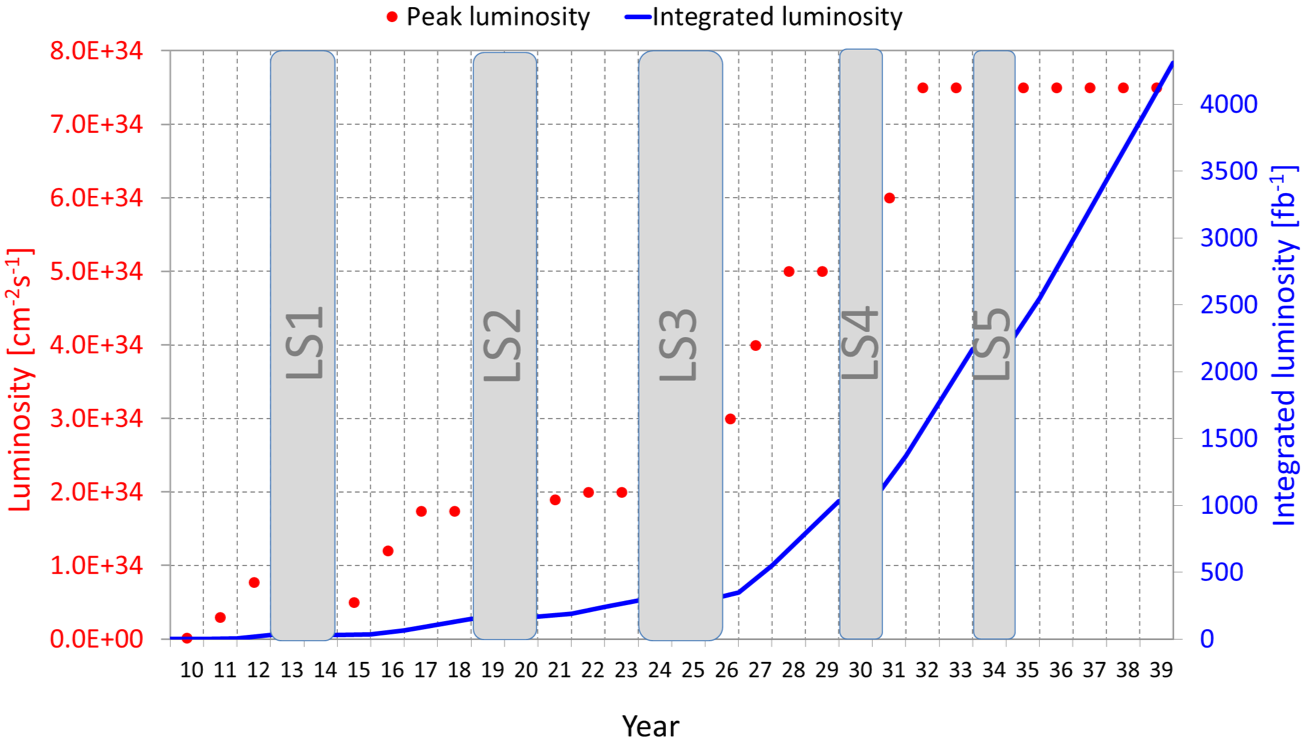
\includegraphics[scale=.35]{Immagini/LHC_lumi_2010_2039.png}
\caption{L'evoluzione della luminosit\`a istantanea e integrata di LHC fino al 2039 con i previsti periodi di interruzione della presa dati; LHCC P 008}
\label{HL-LHC}
\end{figure}

\subsection{Le motivazioni di fisica di HL-LHC}

HL-LHC amplier\`a enormemente il potenziale di fisica di LHC sia per le misure di precisione e per i processi rari nell'ambito del MS, sia per la portata di scoperta di processi previsti da teorie oltre il MS.
 
Un esempio \`e lo studio degli accoppiamenti di Yukawa del bosone di Higgs che, grazie a HL-LHC, potranno essere misurati da CMS con precisioni dell'ordine di qualche percento anche nel caso del muone che, con una frazione di decadimento di $\sim 10^{-4}$, \`e sperimentalmente ambizioso.
Il notevole miglioramento della precisione delle misure degli accoppiamenti del bosone di Higgs \`e illustrato in Fig.~\ref{HLLHCCouplings} nel confronto tra i risultati del RunI e la stima di quanto ottenibile a HL-LHC.
\begin{figure}
\centering
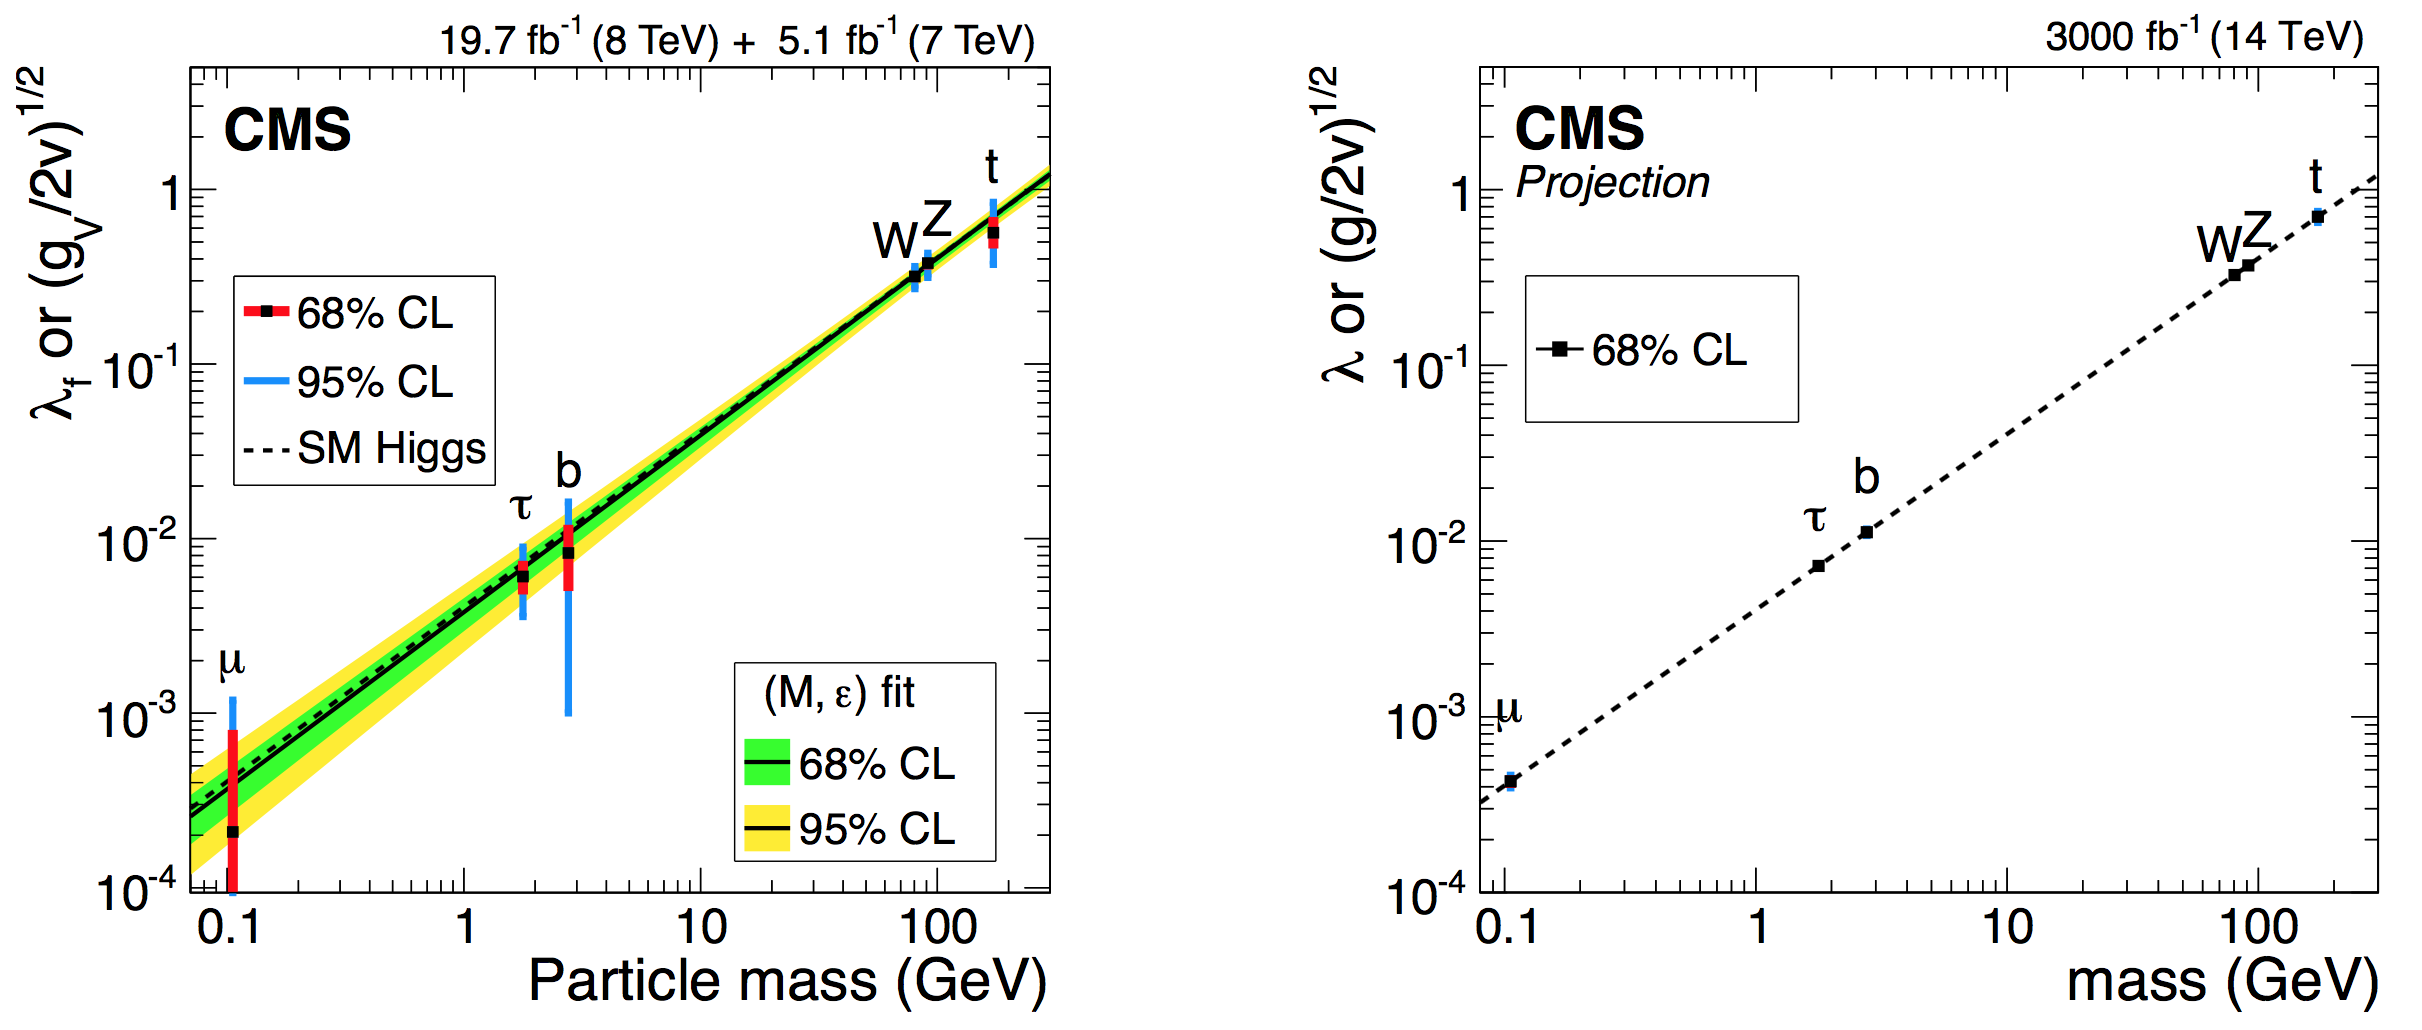
\includegraphics[scale=.35]{Immagini/HLLHC_Couplings.png}
\caption{Gli accoppiamenti del bosone di Higgs a fermioni e bosoni parametrizzati come $(g_V/2v)^{1/2}$, dove $v$ \`e il valore di aspettazione di vuoto de campo di Higgs in funzione della massa della particella; a sinistra le misure effettuate a RunI; a destra con l'estrapolazione delle incertezze a HL-LHC per $3000\ifb$ di luminosit\`a integrata assumendo gli accoppiamenti previsti dal MS.}
\label{HLLHCCouplings}
\end{figure}

Uno studio fondamentale \`e quello della produzione in coppie di Higgs, che permette di investigare i vertici trilineari con cui il bosone di Higgs interagisce con se stesso, come lo studio dei processi di scattering che coinvolgono i bosoni vettori deboli. Tutti questi processi sono intimamente legati alla rottura spontanea ella simmetria elettrodebole e al ruolo del bosone di Higgs stesso nel MS~\cite{vediTDRref13}. Eventuali deviazioni dalle previsioni del MS sarebbero indizio di nuova fisica oltre il MS stesso. Pur rappresentando una difficile sfida sperimentale per i fondi dominanti, se non irriducibili, e le piccole sezioni d'urto HL-LHC ne consentir\`a uno studio approfondito.

In questi ambiti \`e importante notare come la regione in avanti a grande pseudo-rapidit\`a sia sperimentalmente molto attraente perch\'e, dati i processi di produzione, vi si concentra una frazione non trascurabile del segnale. Si veda, a titolo di esempio, la Fig.~\ref{fig:VBFHtt_HH4b} relativa a processi tra i pi\`u interessanti dal punto di vista sperimentale: il processo H$\rightarrow \tau\tau$ in cui l'Higgs \`e prodotto per scattering di bosoni vettori ({\em Vector Boson Fusion}, VBF) e la produzione in coppia di bosoni di Higgs che decadono successivmante in coppie $\mathrm{b}\overline{\mathrm{b}}$, $\mathrm{HH}\rightarrow \mathrm{b}\overline{\mathrm{b}}\mathrm{b}\overline{\mathrm{b}}$. In entrambi i casi una accettanza di rivelazione estesa a grande pseudo-rapidit\`a permetterebbe di incrementare sensibilmente l'accettanza sperimentale per i processi in oggetto.
\begin{figure}[t]
\centering
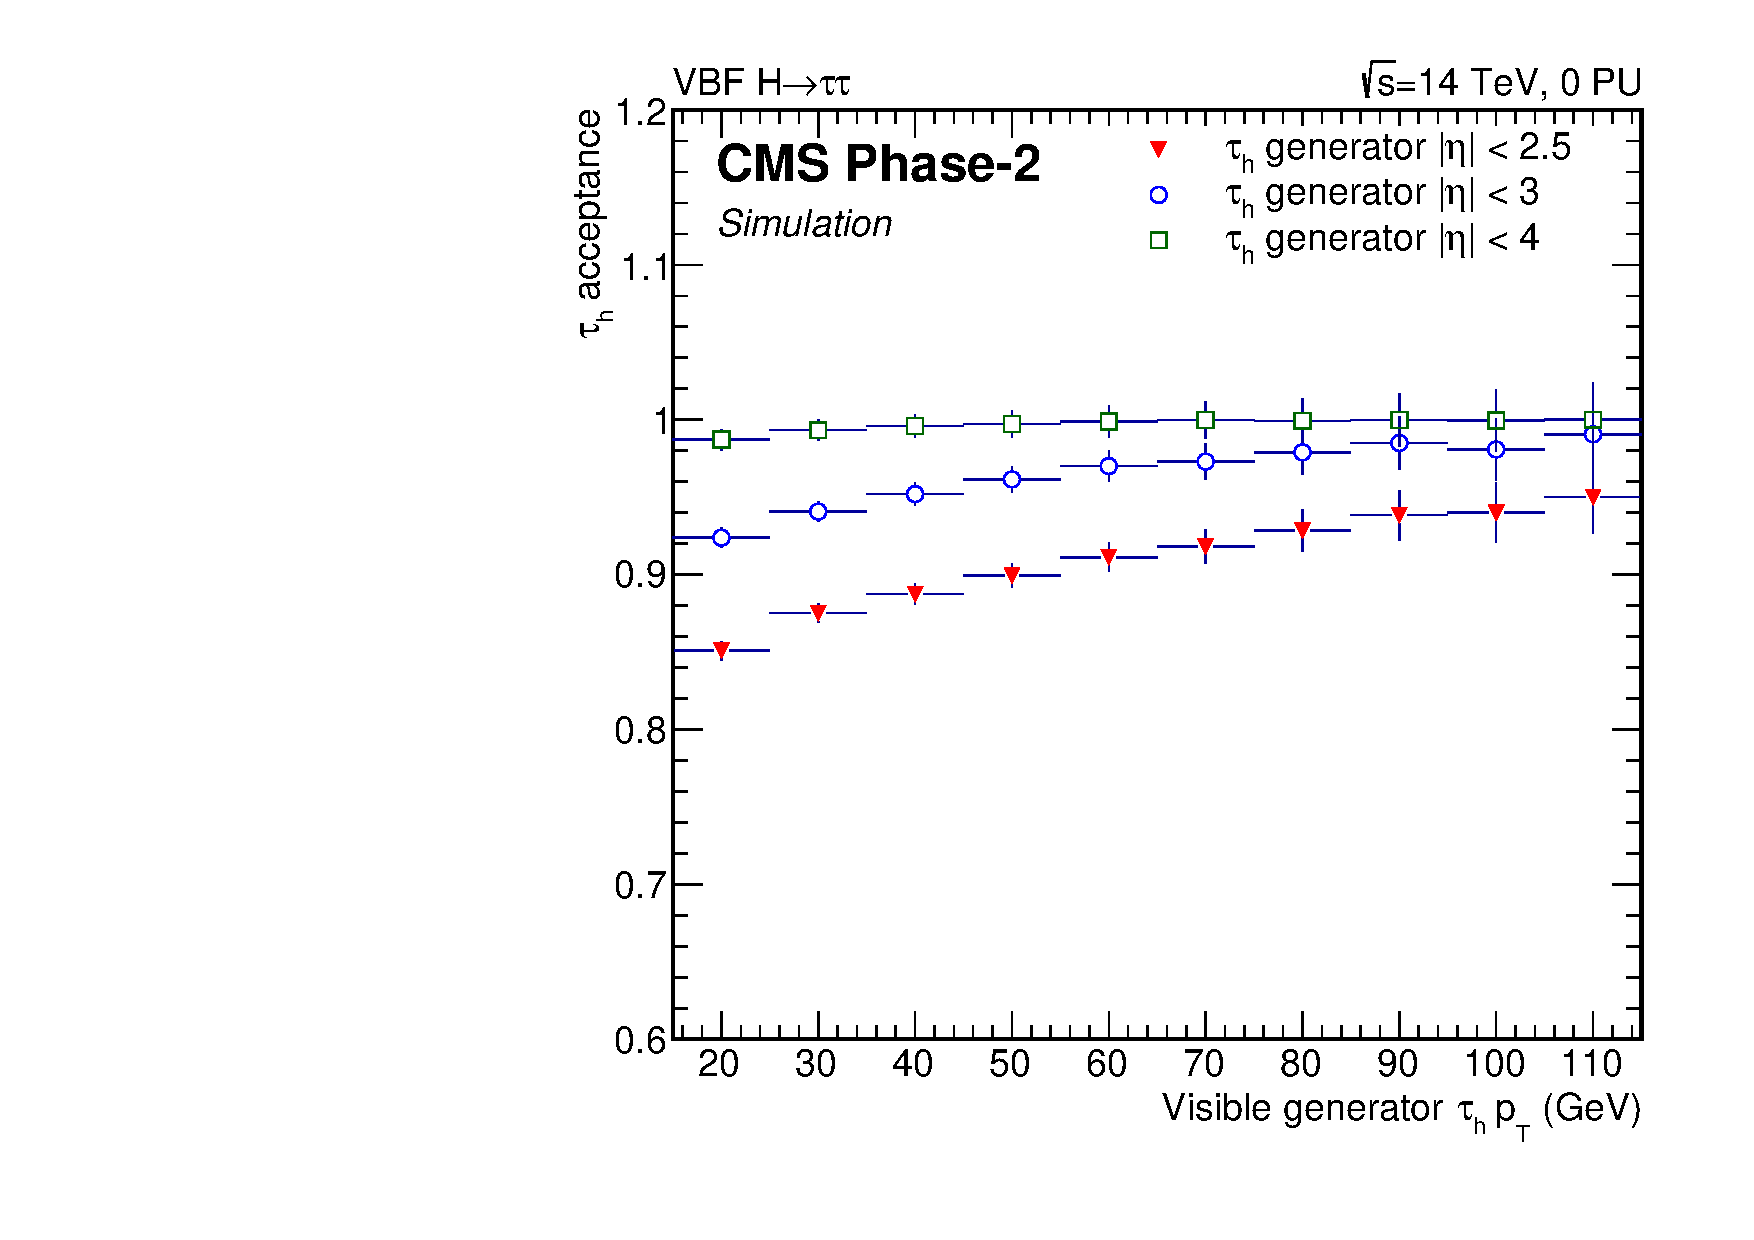
\includegraphics[width=0.45\textwidth]{Immagini/VBF_HTT_tau_acceptance.pdf}
\hfill
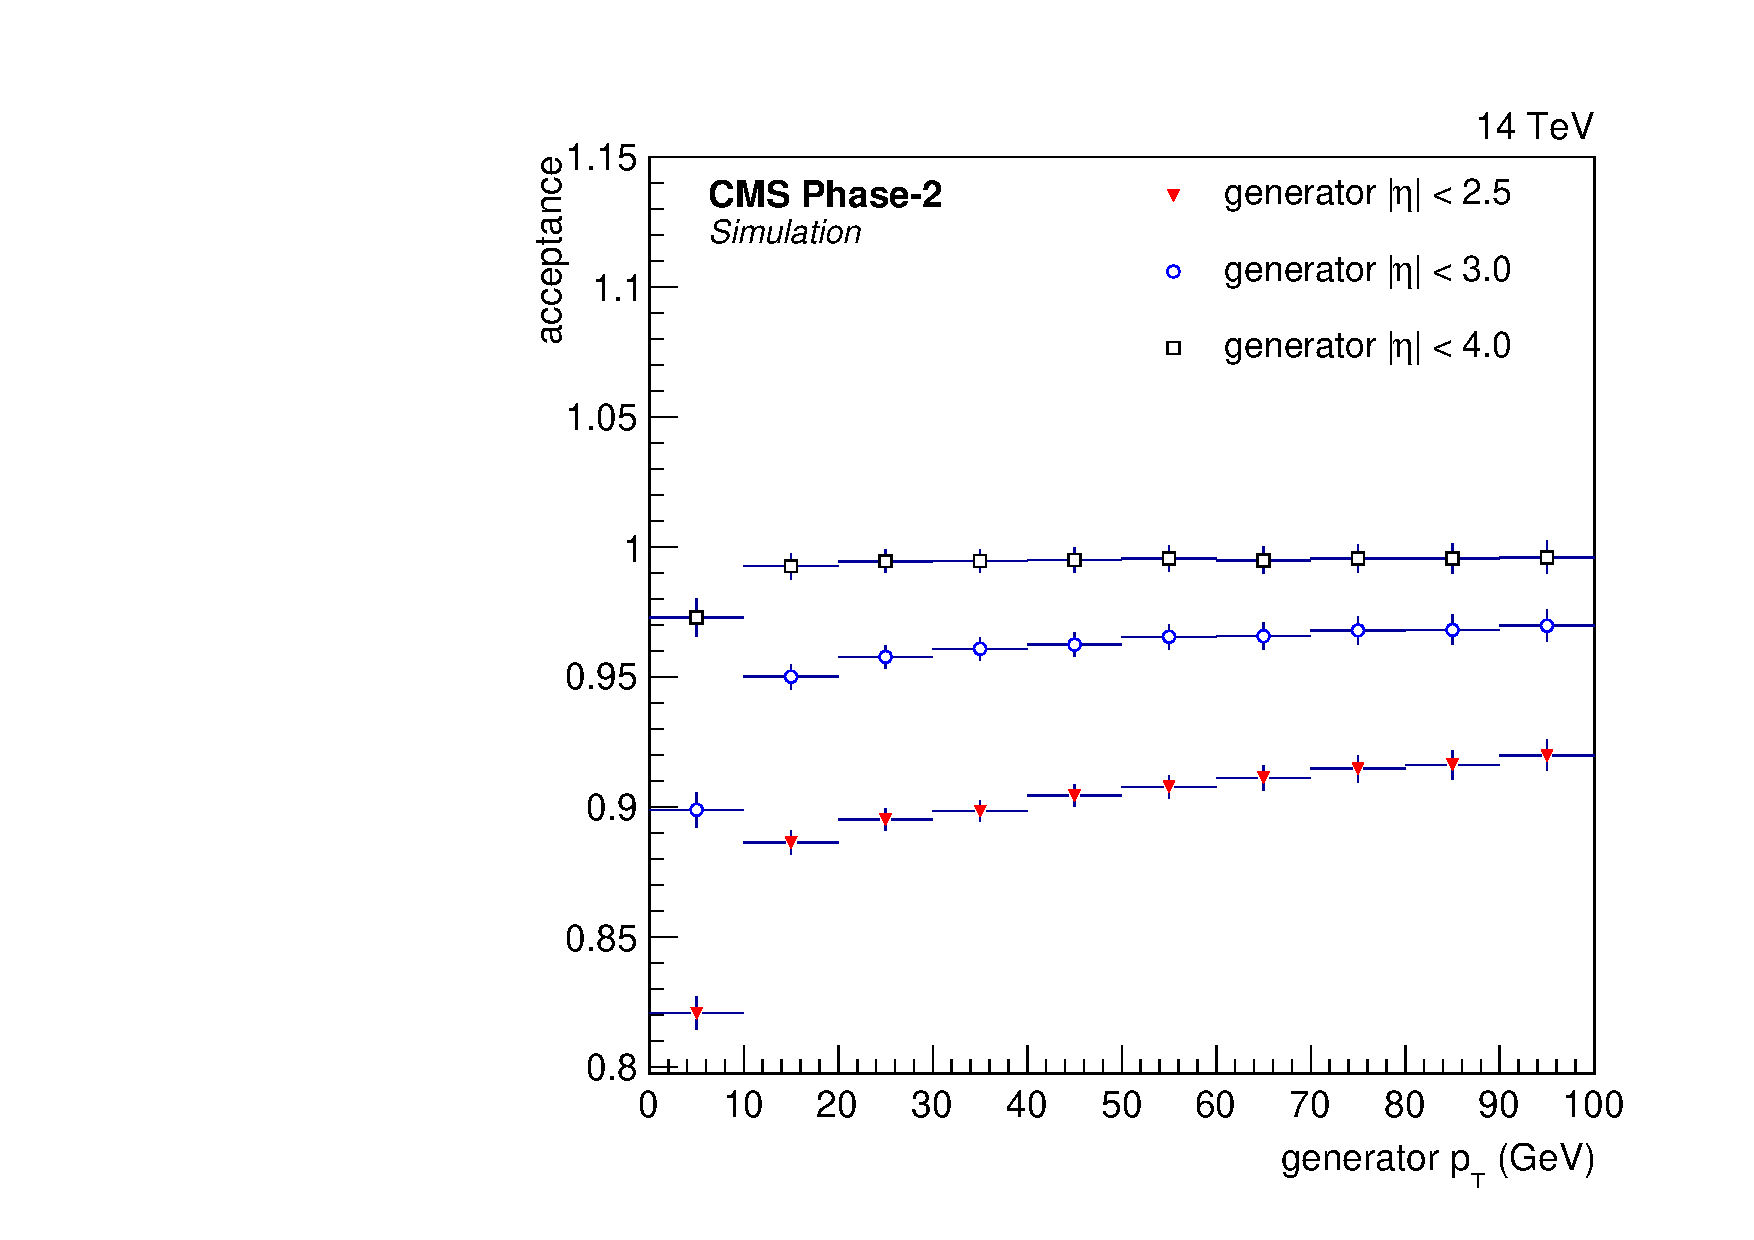
\includegraphics[width=0.45\linewidth]{Immagini/HH4b_acc.pdf}
\caption{Sinistra: accettanza relativa a leptoni $\tau$ che decadono adronicamente, $\tau_{\mathrm{h}}$, in funzione dell'impulso trasverso visibile  $\tau_{\mathrm{h}}$ $\pt$ generato nella simulazione per tre selezioni in pseudo-rapidit\`a; destra: frazione dei b-jet negli eventi di segnale, stimata con la simulazione, in funzione del $\pt$ del jet stesso per tre selezioni in pseudo-rapidit\`a. Per entrambe le figure le selezioni in pseudo-rapidit\`a sono $|\eta|<2.5$ (rosso), $|\eta|<3$ (blue) e $|\eta|<4$ (verde).
}
\label{fig:VBFHtt_HH4b}
\end{figure}

L'aumento di luminosit\`a, rendendo visibili processi con piccola sezione d'urto, amplier\`a il potenziale di scoperta di LHC per le ricerche dirette di nuove particelle previste dai modelli di estensione del MS ({\em beyond standard model} o BSM) inclusi quelli ritenuti pi\`u promettenti come la Supersimmetria e i modelli che prevedono extra-dimensioni o bosoni di gauge alla scala del TeV. Le ricerche indirette di nuova fisica che si basano sulla misura di decadimenti rari godranno di un analogo beneficio. Per esempio l'analisi del canale $B^0_s\to \mu\mu$ diventer\`a una misura di precisione e si stima che l'osservazione del decadimento $B_0\to\mu\mu$ sar\`a statisticamente solida con una significanza statistica di oltre 6 $\sigma$.

% \subsection{Obiettivi}

% L'idea di aumentare la luminosità di LHC oltre quella decisa nel progetto originale è antecedente alla messa in opera del progetto. Eventuali modifiche importanti alla macchina e agli esperimenti possono essere eseguite solo con lunghi periodi di shut down in cui è possibile accedere al tunnel e alle caverne. Per questo motivo è stato deciso un piano temporale che intervalli periodi di presa dati (Run I, Run II etc.) e periodi in cui si ha uno spegnimento completo per lunghi periodi (LS1, LS2, LS3). In figura \ref{HL-LHC} è possibile vedere la suddivisione temporale tra periodi di presa dati e periodi di spegnimento.
% Run I è stato il periodo di presa dati dal 2011 al 2012. Nel primo periodo di stop LS1 LHC è stato modificato al fine di raggiungere energie  nel centro di massa di 13 TeV, per poi arrivare gradualmente a 14 TeV. In questo momento siamo alla fine del Run II, e nell'esperimento CMS si  hanno una media di 25 interazioni per bunch, ciò vuol dire 25 vertici da ricostruire ogni 25 ns. Attraverso modifiche  e miglioramenti apportati nel LS1 e LS2 verrà aumentata la luminosità, questa parte del processo per l'esperimento CMS va sotto il nome di fase-I. Durante il periodo LS3  saranno invece sostituite vari parti degli esperimenti, che a causa del danneggiamento da radiazione saranno deteriorati e nello contemporaneamente verranno sostituiti i quadrupoli di fuocheggiamento con nuovi modelli capaci di incrementare la luminosità. 
% Il periodo che seguirà LS3 sarà chiamato fase II o HL-LHC (High Luminosity LHC). Nello scenario prefissato la lumiosità istantanea sarà di $5 \cdot 10 34 cm^{-2} s^{-1}$ con picchi di $2 \cdot 10 35 cm^{-2} s^{-1}$, in questo modo gli esperimenti saranno in grado di raccogliere una maggiore statistica con una luminosità di $300 fb^{-1}$ ogni anno per 10 anni(250 o 300)?????%at 5 × 10 34 cm − 2 s − 1 from a potential peak value of 2 × 10 35 cm − 2 s − 1 at the beginning of fills,
% %and to deliver 250 fb − 1 per year for a further 10 years of operation. Under these conditions
% In queste condizioni ci sarà una maggiore probabilità di sovrapposizione di interazioni (Pile Up), questa sarà la grande sfida, insieme alla gestione degli effetti di degradazione in cui incorreranno i rivelatori a seguito delle maggiori dosi di radiazione assorbita. Sempre nella figura \ref{HL-LHC} è possibile vedere le proiezioni di luminosità di picco e luminosità integrata.
 
% %The high luminosity period that follows LS3 with the upgraded LHC is referred to here as HL-LHC or Phase-II. The proposed operating scenario is to level the instantaneous luminosity
% %at 5 × 10 34 cm − 2 s − 1 from a potential peak value of 2 × 10 35 cm − 2 s − 1 at the beginning of fills,
% %and to deliver 250 fb − 1 per year for a further 10 years of operation. Under these conditions the event PU will rise substantially to become a major challenge for the experiments, and the performance degradation due to integrated radiation dose will need to be addressed. This Technical Proposal presents the CMS upgrade program for Phase-II. The schedule of beam operations and long shutdowns, together with projections of the peak and integrated luminosities, is shown in Fig. 1.9, and is, of course, subject to change.

\section{L'esperimento CMS}

Il {\em Compact Muon Solenoid} (CMS) [CMS Collaboration The CMS experiment at LHC JINST 08 (2008) 03] \`e un esperimento polivalente per lo studio generale delle collisioni pp fino ad un’energia di $14\TeV$. Il rivelatore \`e infatti ottimizzato per misurare energia e impulso delle particelle prodotte durante le collisioni. Per garantire la massima ermeticit\`a, l’apparato sperimentale ha una struttura centrale approssimativamente cilindrica, detta {\em barrel}, sigillata ad entrambe le estremit\`a da strutture di chiusura dette {\em endcap} per un diametro complessivo di $15\m$, una lunghezza di $\sim22\m$ e $\sim 12500$ tonnellate di peso. La capacit\`a di identificazione delle particelle prodotte \`e assicurata dai diversi tipi di sotto-rivelatori disposti in strati rispetto al punto di incrocio dei fasci come schematicamente mostrato in Fig.~\ref{fig:spaccatoCMS}: pi\`u internamente i tracciatori di particelle cariche ovvero il rivelatore a pixel di silicio e il rivelatore a microstrip di silicio; all'esterno di quest'ultimo abbiamo il calorimetro elettromagnetico e il calorimetro adronico; il tracciatore e i calorimetri sono collocati all’interno del magnete solenoidale superconduttore che genera un campo magnetico di $3.8\T$ parallelo all'asse dei fasci. Pi\`u esternamente, immerse nel ferro del giogo di ritorno del magnete, si trovano le camere a muoni.
\begin{figure}
\centering
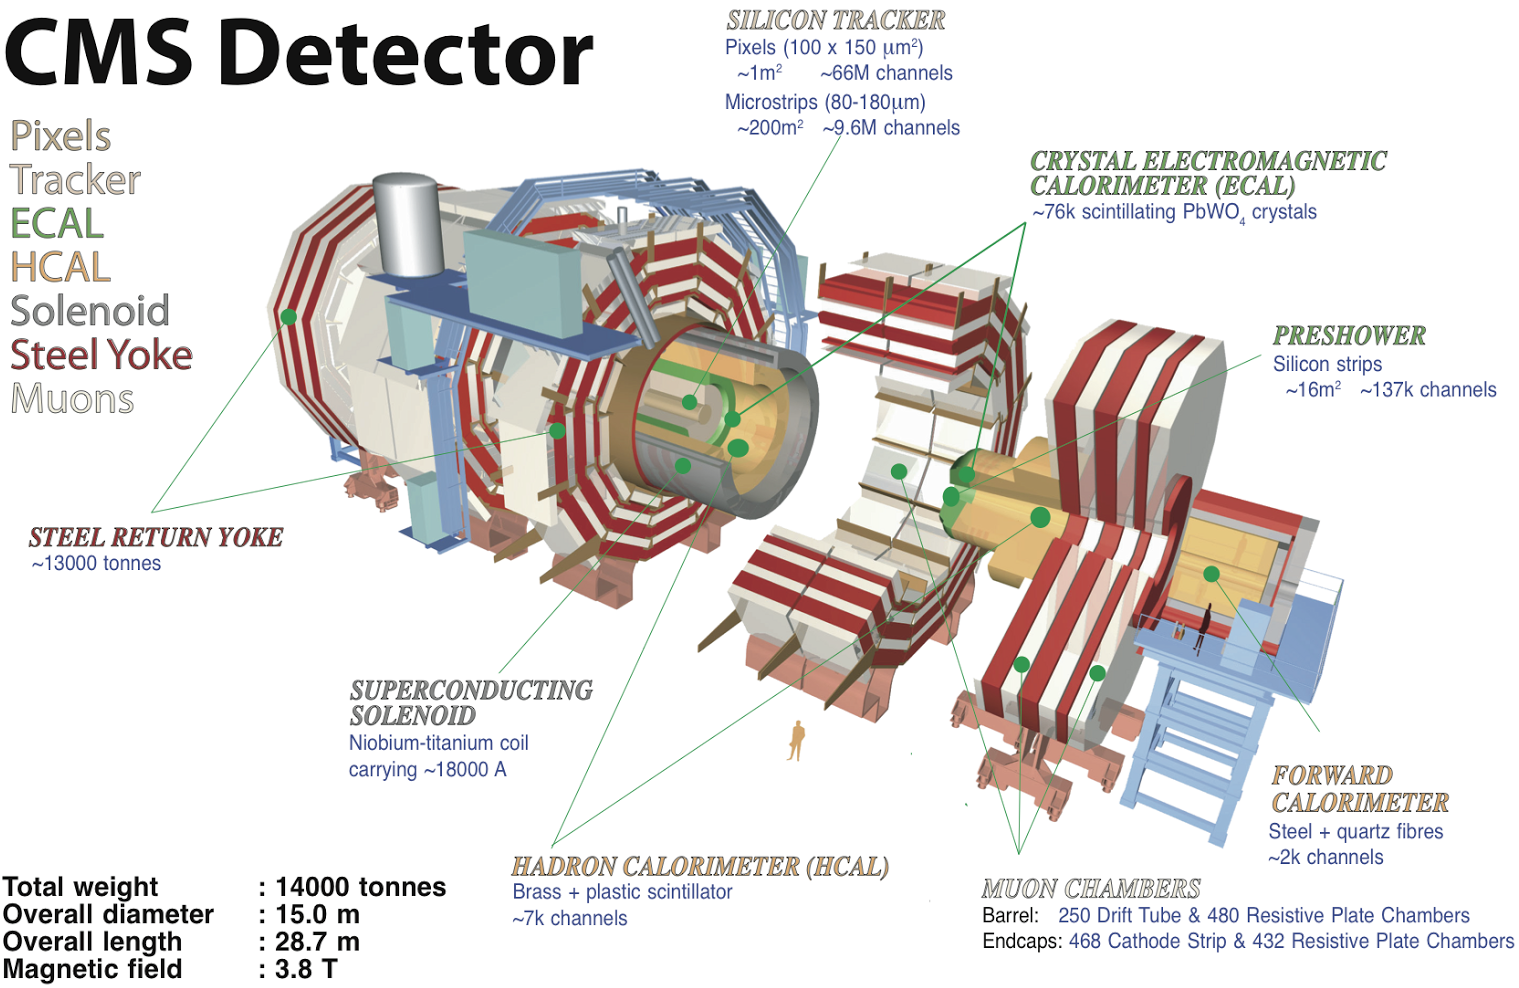
\includegraphics[width=\textwidth]{Immagini/cms_3d.png}
\caption{Vista dello spaccato dell'attuale esperimento CMS in cui sono schematicamente visibili i vari sotto-rivelatori.}
\label{fig:spaccatoCMS}
\end{figure}

L’esperimento \`e collocato in una caverna alla profondit\`a di $\sim 100 m$ in corrispondenza del punto di interazione numero 5 di LHC (IP5). 

Pi\`u nel dettaglio gli attuali sotto-sistemi dell'esperimento CMS sono i seguenti, procedendo dal punto di interazione verso l'esterno:

\begin{description}
\item[Il tracciatore al silicio.] L'apparato in grado di ricostruire la traiettoria delle particelle cariche fino a $|\eta|<2.5$ misurandone l'impulso trasverso (grazie alla presenza del campo magnetico dato che $\pt [\GeV] = 0.3 B [\T] \rho [\m]$, dove $\rho$ \`e il raggio di curvatura) e individuando i vertici primari di interazione pp e gli eventuali vertici secondari di decadimento di particelle instabili prodotte dall'interazione; occupa il volume $r<1.2\m$, $|z|<250\cm$. \`E composto da due sottorivelatori: un rivelatore di vertice a pixel di silicio e un rivelatore a microstrip di silicio. Si veda la sezione~\ref{} per maggiori dettagli.
\item[ECAL.] Il calorimetro elettromagnetico (ECAL) misura l’energia di elettroni e fotoni fino a $|\eta|<3$. Collocato esternamente al tracciatore, \`e un calorimetro omogeneo composto da $\sim 76000$ cristalli scintillanti di tungstato di piombo (PbWO$_4$) di lunghezza equivalente a $\sim 25--26X_0$.
\item[HCAL.] Il calorimetro adronico (HCAL) misura l'energia delle particelle che interagiscono adronicamente fino a $|\eta|<5$ ed \`e. \`E un calorimetro ermetico a campionamento situato a valle di ECAL, rispetto al punto di interazione, composto da strati di ottone e di scintillatore plastico, corrispondenti a $7-11$ lunghezze d'interazione, e integrato da uno strato di scintillatore posto all'esterno del magnete nella parte barrel che ne aumenta lo spessore efficace per il contenimento degli sciami adronici.
\item[Il magnete superconduttore.] Il campo magnetico che deflette le particelle cariche cos\`i da stimarne l’impulso dalla curvatura \`e generato da un magnete superconduttore solenoidale lungo $13\m$, con un diametro interno di $6\m$, costituito da un un avvolgimento di cavo di NbTi in matrice di alluminio mantenuto alla temperatura di $4\degrees\K$ da un sistema criogenico. Il campo magnetico ha una intensit\`a nominale di $3.8\T$ corrispondenti a $\sim 20\kA$ di corrente,  di intensit\`a richiede circa $20\kA$ di corrente. Le linee di campo sono richiuse tramite un giogo esterno di $10000$ tonnellate di ferro.
\item[Le camere a muoni.] Il giogo di ritorno del magnete \`e attrezzato con rivelatori dedicati alla tracciatura dei muoni grazie anche al campo residuo di $1.8\T$ presente nel giogo. Nella parte barrel ci sono camere a deriva ({\em drift chamber}) e CSC ({\em cathode strip chamber}) negli endcap, in entrambi i casi integrati con RPC ($resistive plate chamber$).  
\end{description}

Una rappresentazione schematica dei differenti meccanismi di interazione delle varie particelle nei sotto-rivelatori, sui quali l'identificazione delle stesse \`e basata, \`e visibile in Fig.~\ref{fig:spicchioCMS}.
\begin{figure}
\centering
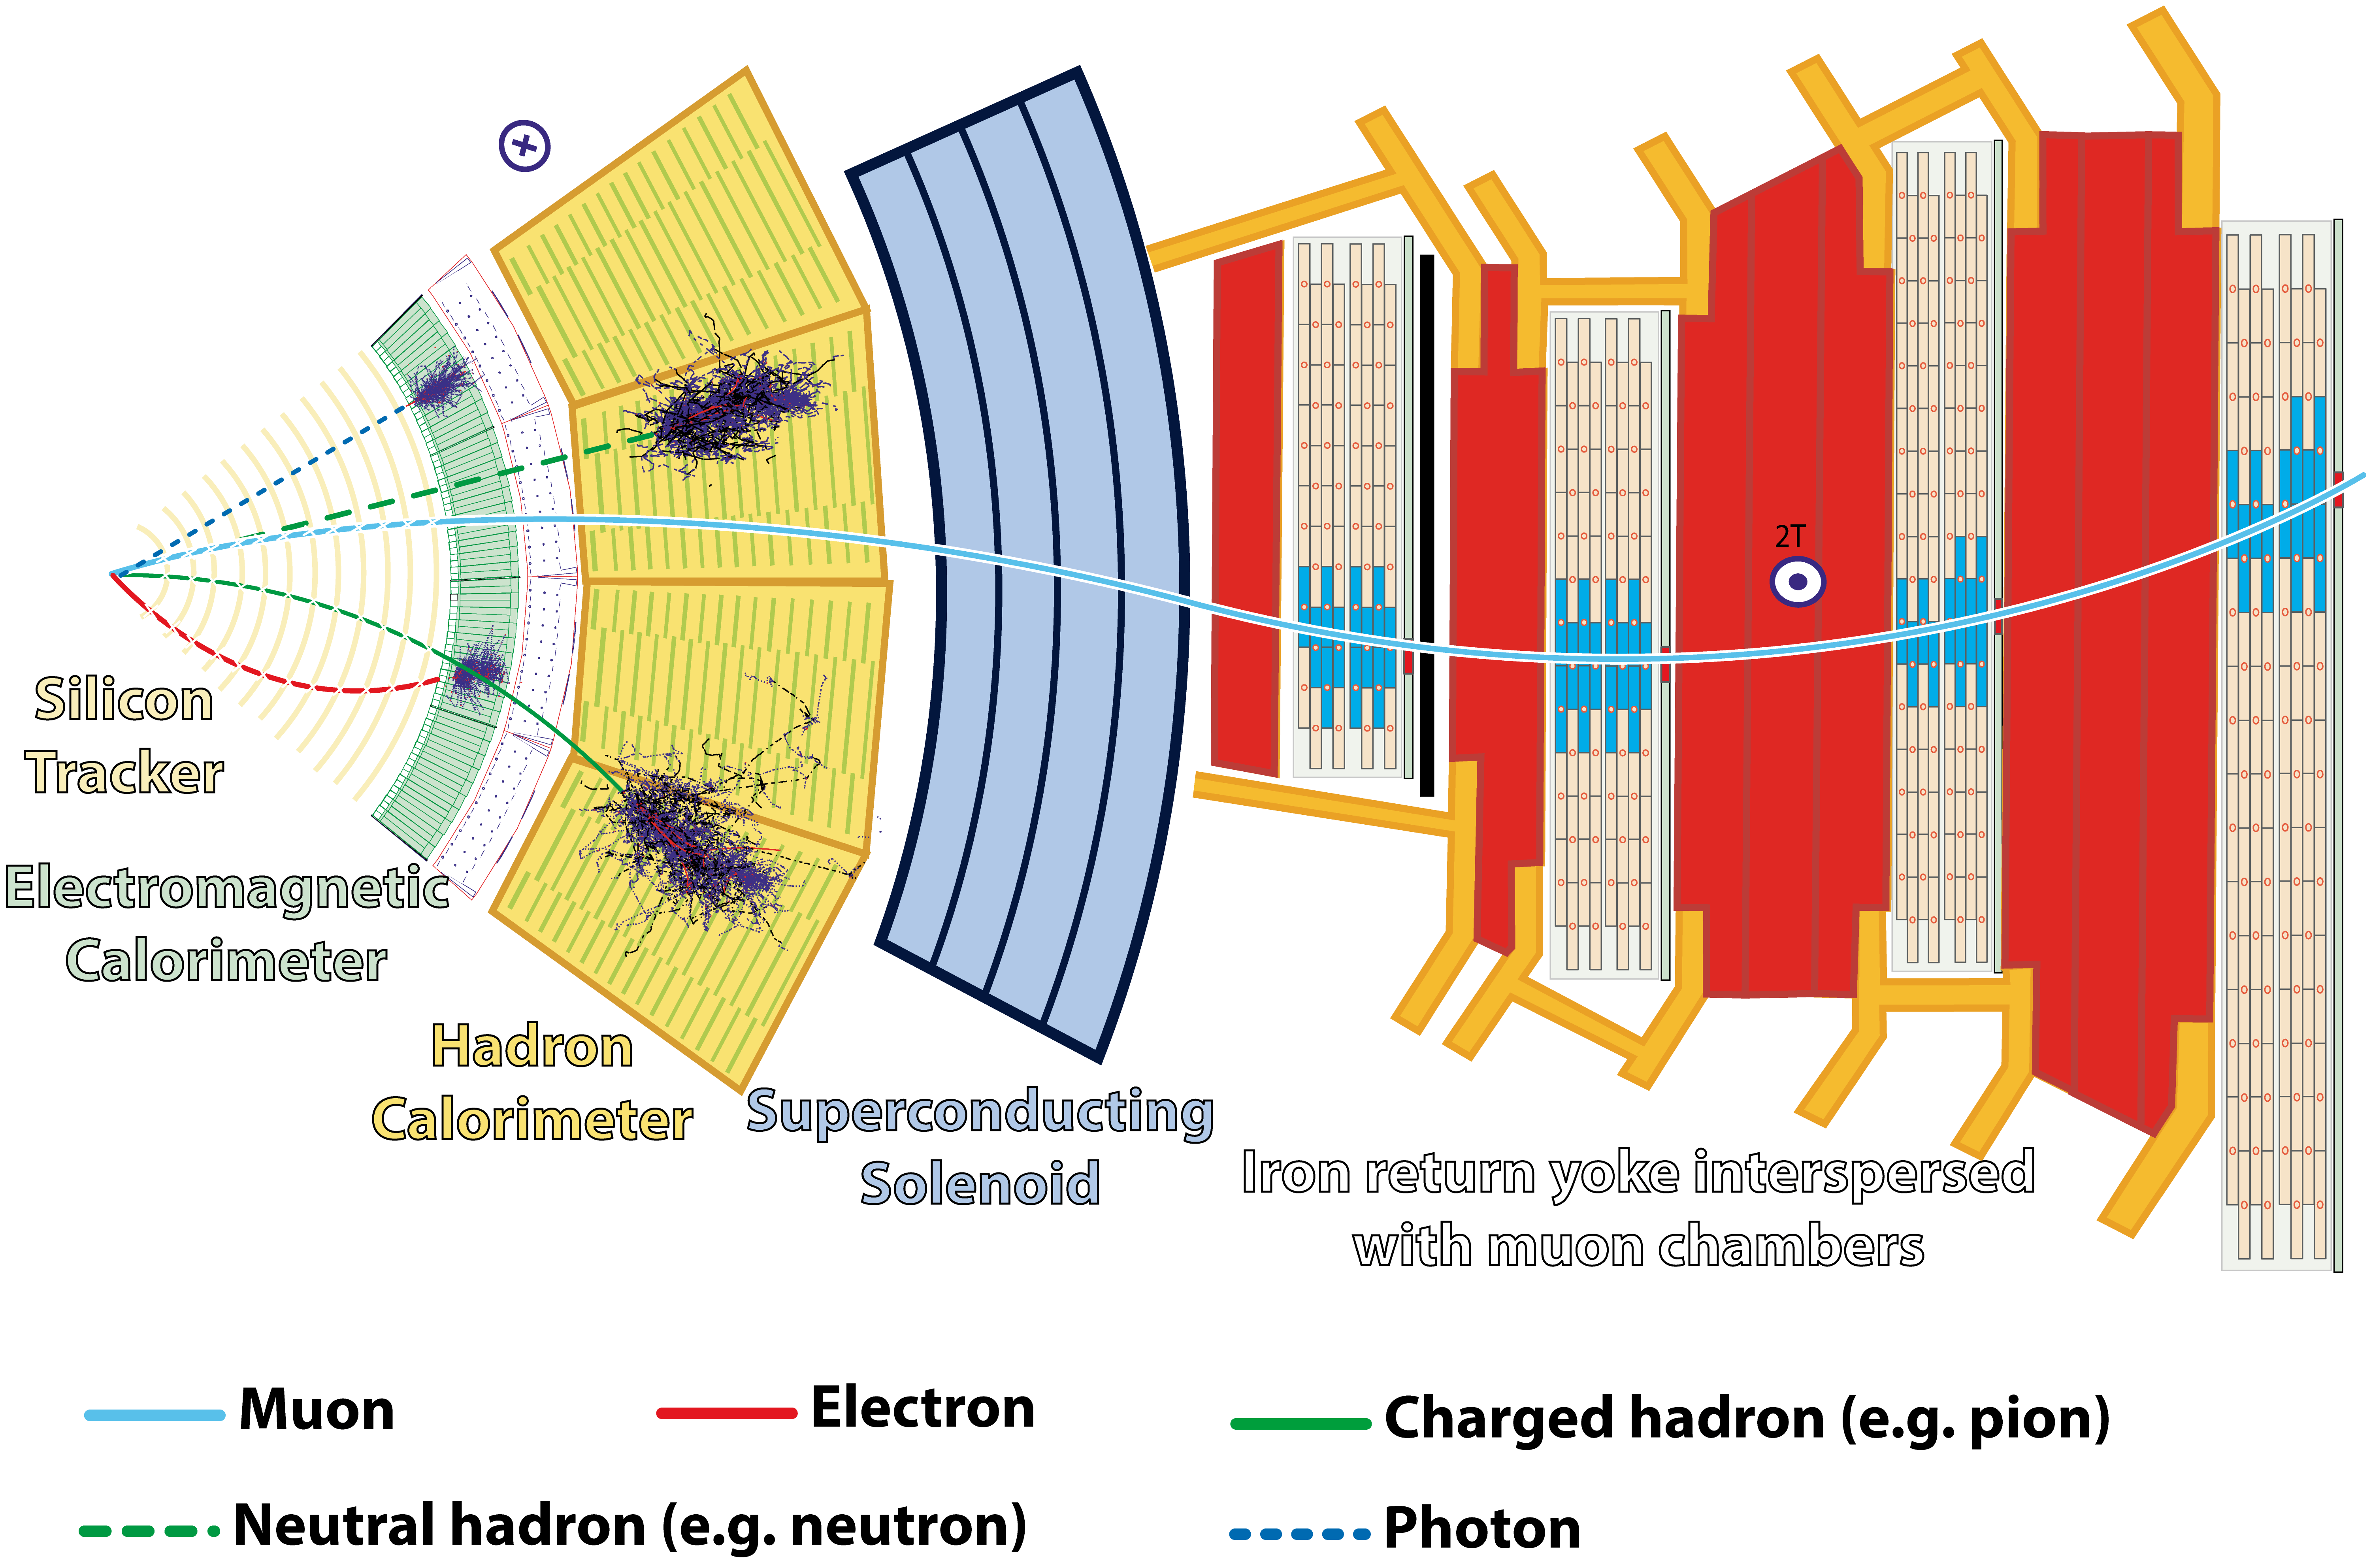
\includegraphics[scale=0.8]{Immagini/CMSbis}
\caption{Spaccato di CMS e risposta ai vari tipi di particella.}
\label{CMSbis}
\end{figure}

La frequenza di $40\MHz$ con cui avvengono i bunch crossing a LHC rende impraticabile il trasferimento integrale per ogni evento dei dati relativi ai $>100$M di canali di lettura di tutto CMS ({\em readout}). Sarebbe inoltre impossibile l'immagazzinamento di questa informazione data l'entit\`a delle memorie di massa che sarebbero richieste. Gli eventi di collisione sono quindi preventivamente filtrati da un sistema di {\em trigger} organizzato in due livelli di crescente complessit\`a che permettono di selezionare gli eventi interessanti per la fisica rispettando le limitazioni del readout e dell'archiviazione a lungo termine dei dati raccolti.

Il primo livello, detto {\em trigger di livello 1} (L1), sfrutta una lettura speciale a bassa risoluzione e granularit\`a dei rivelatori intrinsecamente veloci, ovvero calorimetri e camere a muoni. Questa informazione viene elaborata entro pochi microsecondi ({\em latenza}) compatibilmente con la profondit\`a temporale delle memorie tampone ({\em pipeline}) dell'elettronica di lettura di prossimit\`a ({\em front-end}) di tutti i sotto-rivelatori, che immagazzinano i dati in attesa dell'esito della selezione di L1. Questa \`e basata su semplici tagli sulle osservabili fisiche ricavabili dai dati disponibili al sistema di trigger di L1. La frequenza media di consenso del L1 \`e dell'ordine di qualche decina di $\kHz$.

Con il consenso di L1 tutta l'informazione di CMS relativa all'evento selezionato viene letta, digitalizzata e compressa. L'evento, che a questo punto ha una dimensione di $\sim2$MB, viene indirizzato all'{\em High Level Trigger}, HLT. L'HLT \`e una batteria di normali PC commerciali che, grazie alla pesante parallelizzazione e all'utilizzo di flessibili algoritmi semplificati, sono in grado di analizzare e filtrare ulteriormente gli eventi in tempo reale selezionando, con una frequenza media di qualche centinaio di Hz, quelli meritevoli di essere registrati indefinitamente per l'analisi.

%-------------------------

% Questa struttura rispecchia la necessità di ricostruire con precisione gli eventi originati dalla collisione di particelle, che avvengono in rapida successione. CMS come anche gli altri esperimenti, può essere paragonato ad una gigantesca macchina fotografica che registra 40 milioni di foto al secondo (digitalizzando l'informazione di decine di milioni di sensori). 
% La struttura a strati consente di avere rivelatori diversi in ogni strato, di cui i più interni sono meno densi, mentre i più esterni sono più densi. Questo perché il tracciatore non deve alterare l'energia delle particelle che poi sarà misurata nei calorimetri e per facilitare la ricostruzione delle tracce è importante evitare fenomeni di multiple scattering.

% Le particelle che gli scienziati cercano di riprodurre nelle collisioni protone-protone hanno vite medie molto brevi, e decadono rapidamente in particelle più leggere. Dopo un processo di hard-scattering migliaia di queste particelle leggere sono generate elettroni, muoni, fotoni, ma anche protoni, neutroni etc. Tutte queste particelle attraversano i vari strati di cui è composto il rivelatore. 
% Le informazioni raccolte vengono utilizzate per ricostruire l'evento di interazione, per  dedurre l'esistenza di nuove particelle.


% Le traiettorie delle particelle cariche sono piegate dal campo magnetico, e il loro raggio di curvatura è utilizzata per calcolare il loro impulso: maggiore è la loro energia cinetica, minore è la curvatura. Un'altra componente importante di un rivelatore sono i calorimetri per misurare l'energia delle particelle (sia cariche che non). 
% I calorimetri devono essere abbastanza grandi per assorbire anche le particelle più energetiche. Questi motivi fanno sì che gli esperimenti ad LHC siano così grandi. I rivelatori sono costruiti in modo il più possibile ermetico per raccogliere tutti i prodotti delle interazioni e poter ricostruire gli eventi. 
% Combinando le informazioni di ogni strato del rivelatore è possibile determinare il tipo di particella che ha lasciato una data traccia.

% Particelle cariche come elettroni, protoni e muoni, lasciano tracce ionizzando il materiale attraversato. Gli elettroni sono molto leggeri e perciò perdono energia velocemente, mentre i protoni penetrano più in profondità negli strati del rivelatore. I fotoni essendo neutri non rilasciano segnali nel tracciatore, ma nei calorimetri sono convertiti in elettroni e positroni e così ne viene misurata l'energia. 
% L'energia dei neutroni viene invece misurata indirettamente, trasferiscono l'energia ai protoni, che poi sono misurati. I muoni insieme ai neutrini (che non vengono rivelati) sono i soli a raggiungere gli strati più esterni.


% Ogni parte del rivelatore è connessa ad un sistema di lettura elettronico attraverso migliaia di cavi. Ogni volta che un segnale è raccolto, il sistema registra la sua posizione e l'istante in cui è stato raccolto, se il sistema di trigger decide che l'evento che ha generato Se tale segnale è di interesse, allora l'informazione è letta e portata all'esterno del rivelatore per essere utilizzata nelle analisi offline.
% Ci sono differenti criteri per selezionare un evento potenzialmente di interesse, in questo modo la mole enorme di eventi registrati in un secondo viene ridotta a poche centinaia, che poi verranno analizzate in dettaglio.


\subsection{L'attuale Tracciatore al Silicio di CMS}

Il tracciatore al silicio di CMS attualmente istallato merita una descrizione pi\`u approfondita per introdurre le motivazioni e i miglioramenti del potenziamento previsto per HL-LHC oggetto di questo lavoro di tesi.

Il tracciatore al silicio \`e il rivelatore di CMS pi\`u interno: \`e lungo $\sim6\m$ e ha un diametro esterno di $\sim 2.6\m$ ed \`e composto da un barrel centrale e da due endcap finali in modo tale da avere la massima ermeticit\`e fino a $|\eta|<2.5$.

La particella carica rilascia energia nel sensore di silicio che non \`e altro che un diodo contropolarizzato, per avere un volume di raccolta essenzialmente privo di portatori di carica. La carica di ionizzazione che segue al rilascio di energia viene raccolta dagli elettrodi di giunzione. Un elettrodo di giunzione finemente segmentato permette di avere informazione sulla posizione di passaggio della particella carica.

Il disegno del tracciatore \`e caratterizzato da: un’alta granularit\`a, soprattutto vicino al punto di interazione, dove il flusso di particelle \`e maggiore, per avere risoluzione in impulso e un'ottima ricostruzione di tracce limitando, in media, la frazione di canali interessati dal segnale ({\em occupancy}); un elevato e ridondante numero di punti misurati per traccia, per mitigare le conseguenze di possibili malfunzionamenti.
% una quantit`a non eccessiva di materiale da attraversare, che deteriora la precisione delle misure a causa dei fenomeni di scattering multiplo e della perdita di energia nel materiale.
Il tracciatore di CMS, schematicamente rappresentato in Fig.~\ref{fig:CMSTk}, \`e infatti composto di due sotto-rivelatori: il rivelatore a pixel con sensori pi\`u segmentati all'interno e il rivelatore a microstrip pi\`u esternamente. 
  
\begin{figure}
\centering
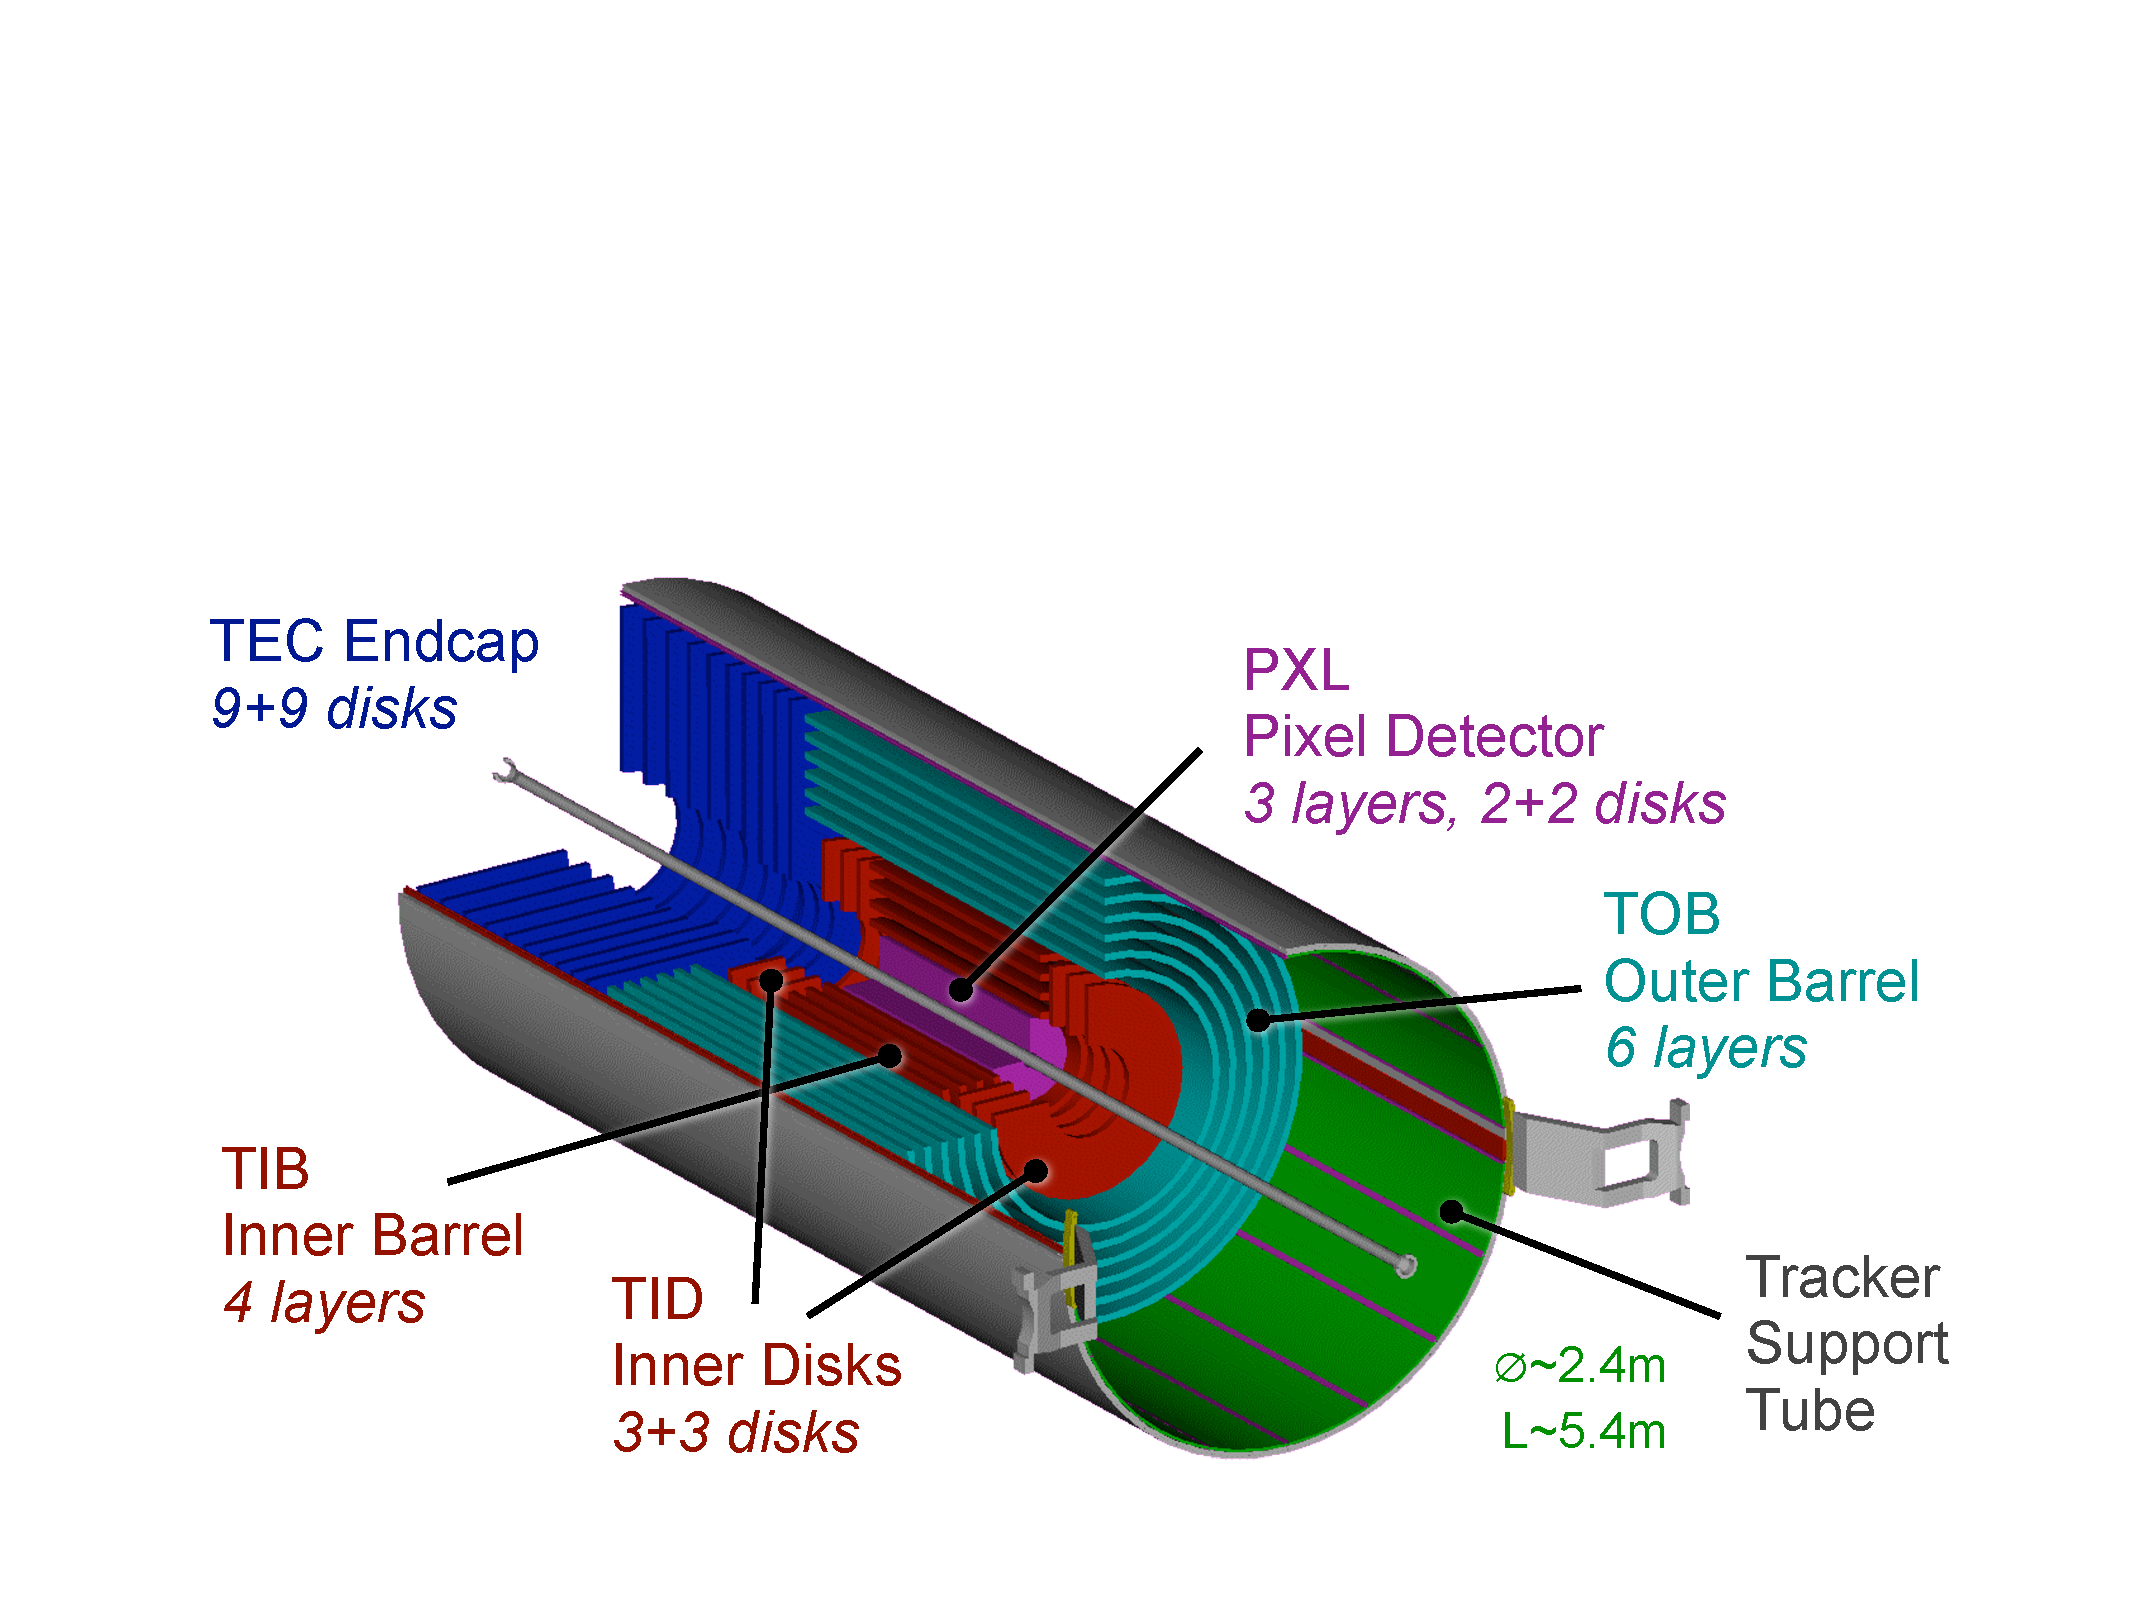
\includegraphics[width=0.45\textwidth]{Immagini/sketch.pdf}
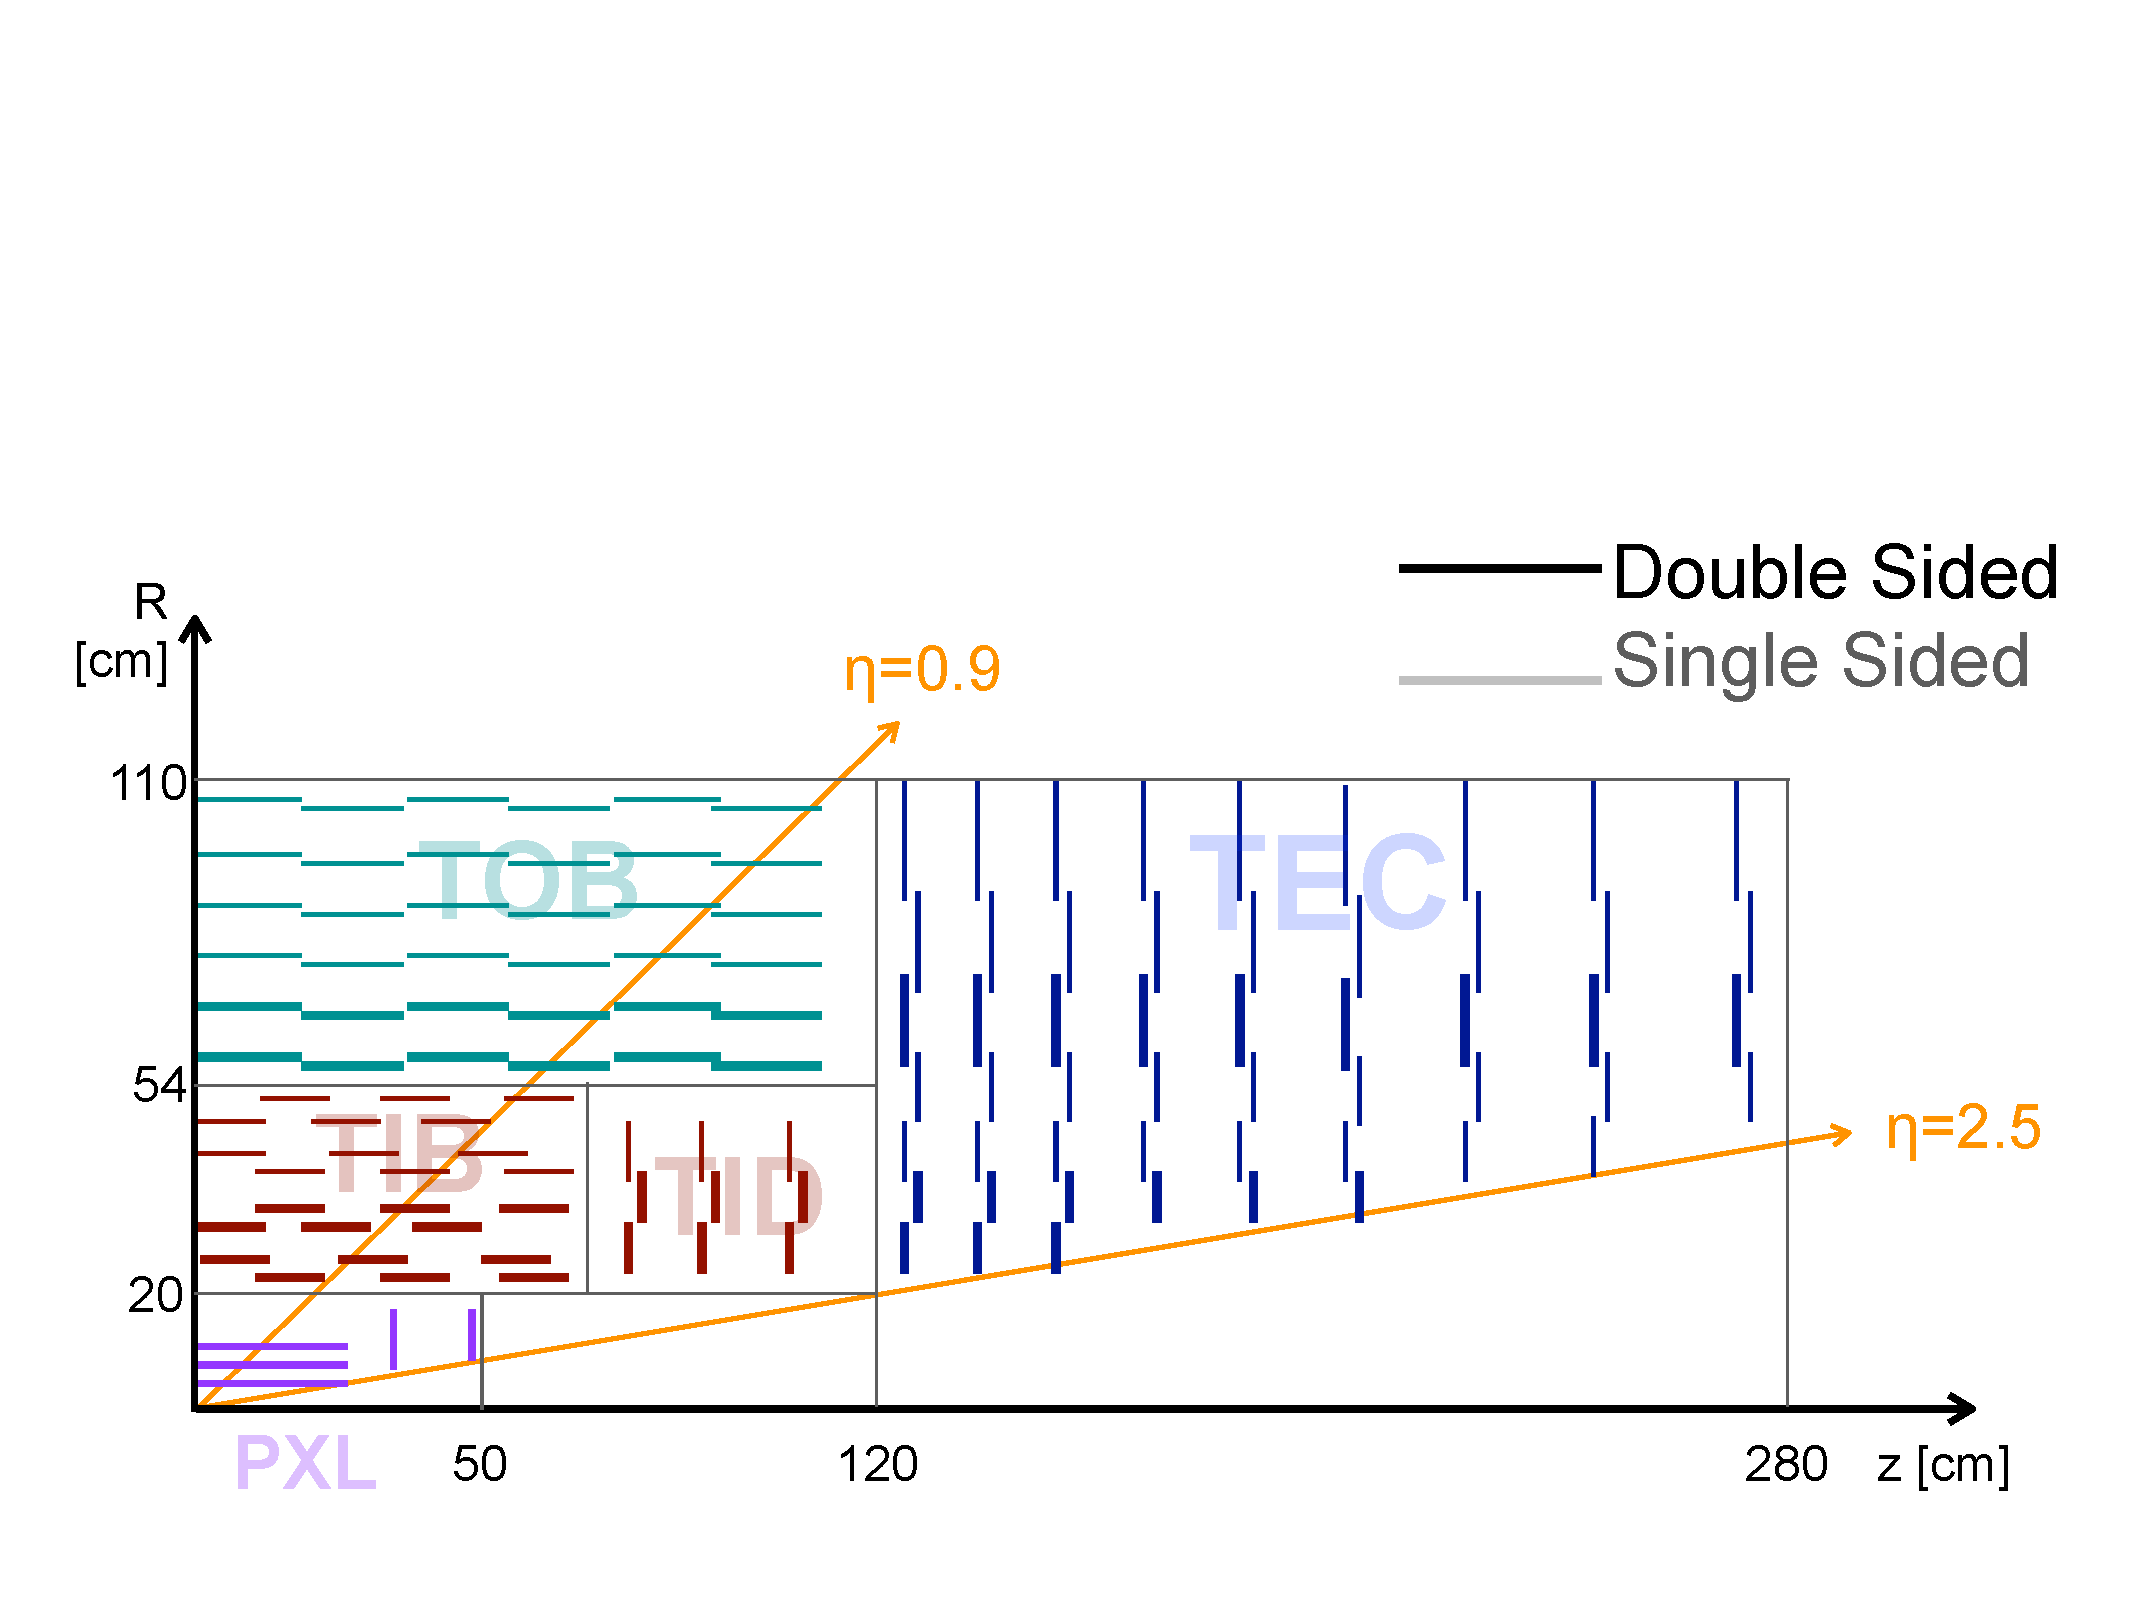
\includegraphics[width=0.45\textwidth]{Immagini/layout_rz.pdf}
\caption{A sinistra: schema semplificato del tracciatore di CMS; a destra: vista $Rz$ di un quadrante del tracciatore di CMS con il primo pixel detector.}
\label{fig:CMSTk}
\end{figure}

Una vista di CMS durante l'istallazione del tracciatore \`e visibile in~Fig.~\ref{fig:CMS}.
\begin{figure}
\centering
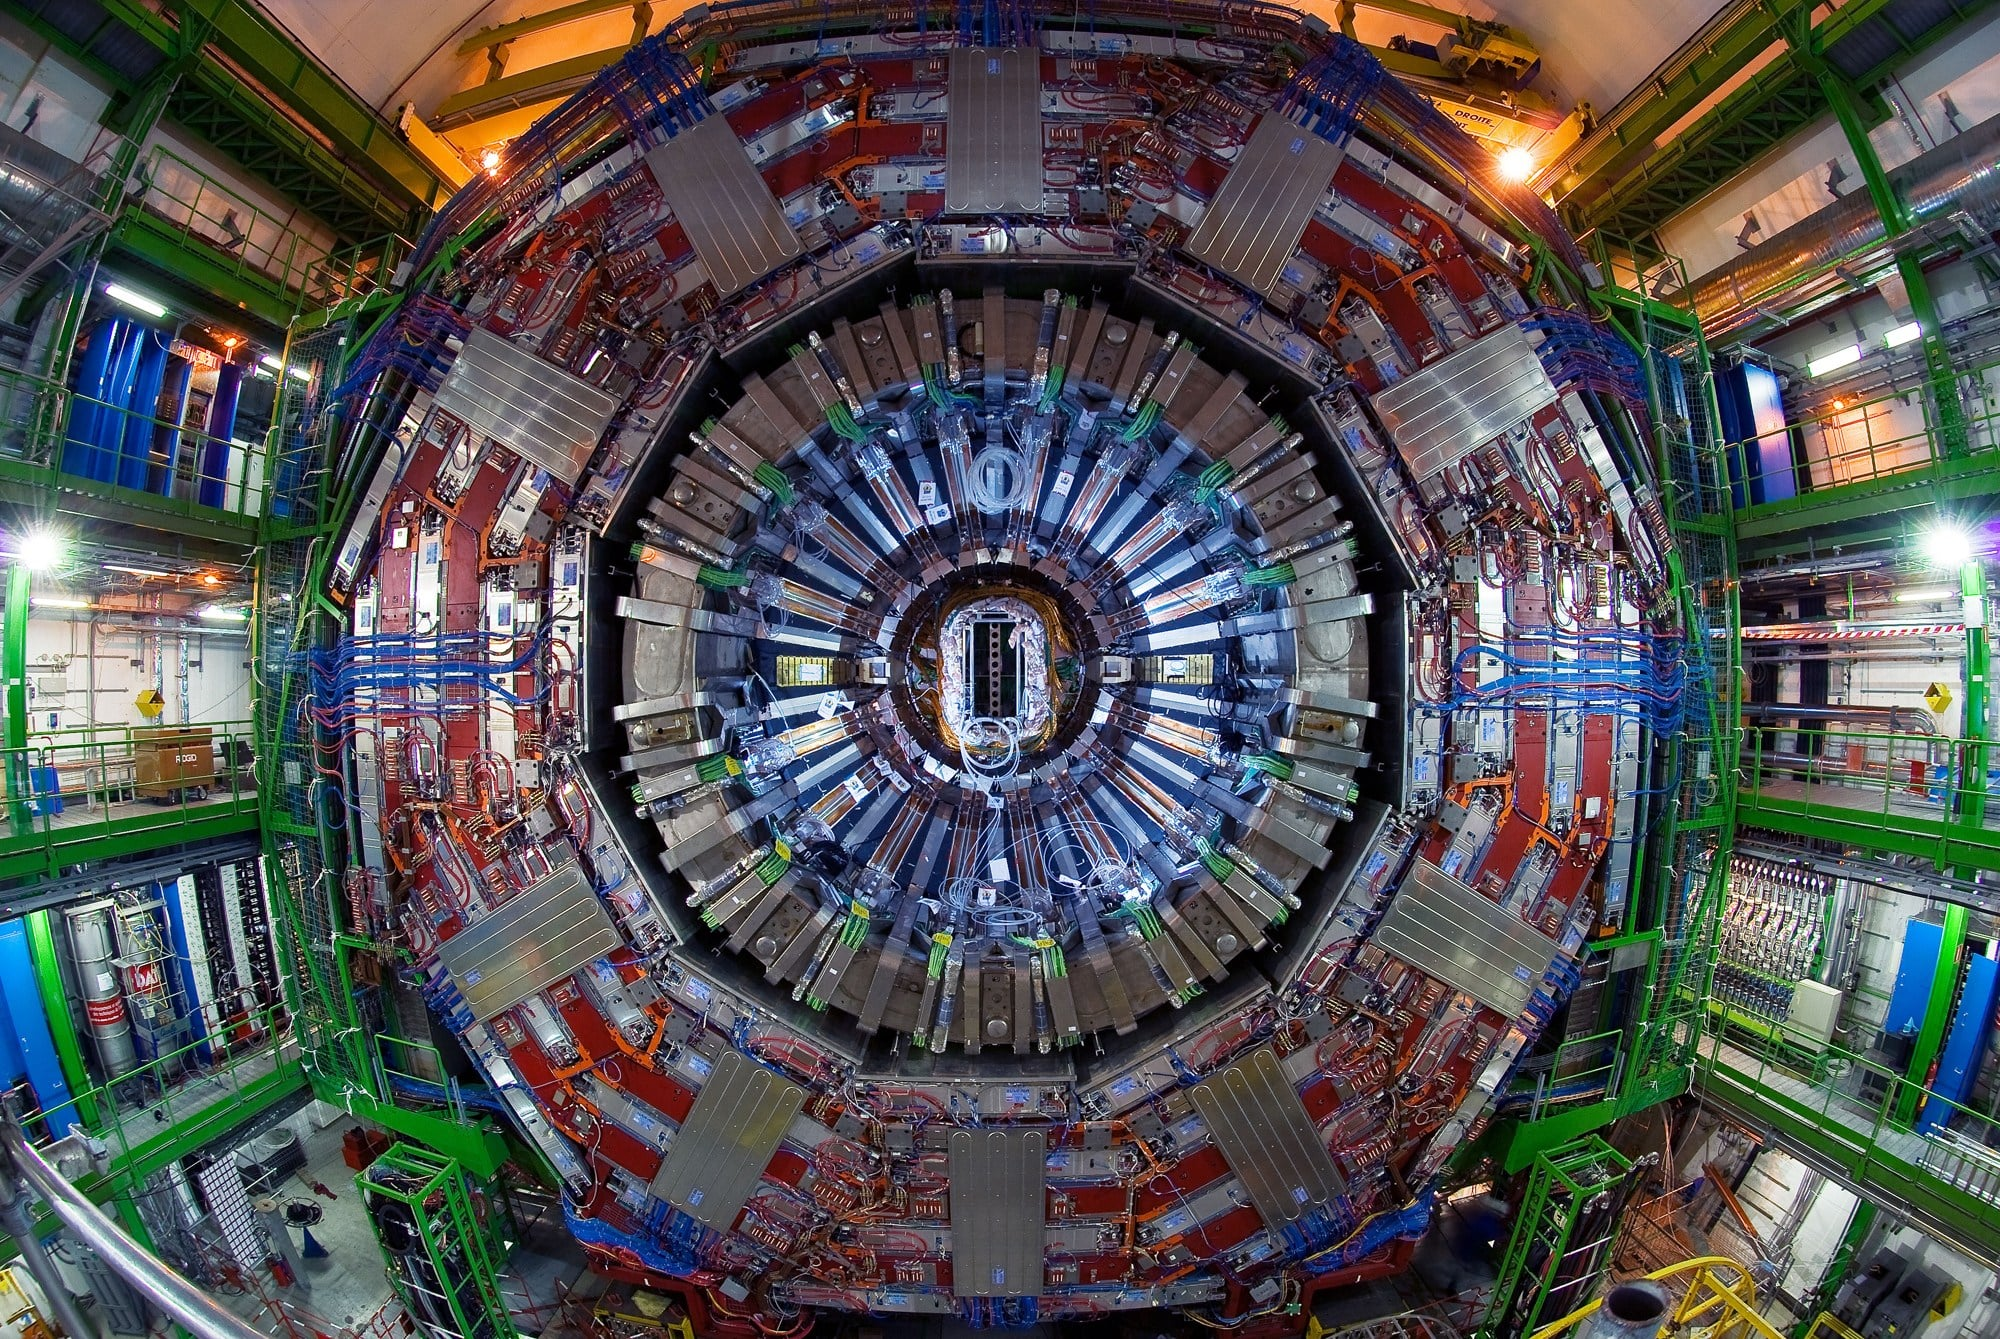
\includegraphics[scale=.2]{Immagini/CMS}
\caption{Vista frontale di CMS durante l'installazione del tracciatore.}
\label{fig:CMS}
\end{figure}

\begin{description}

\item[Il rivelatore a pixel.] Detto anche {\em rivelatore di vertice}, \`e il primo rivelatore che si incontra uscendo dal punto di collisione. CMS ha utilizzato una prima versione del rivelatore di pixel (detta di {\em fase-0}) fino al 2016. A partire dal 2017 \`e operativa una seconda versione evoluta e migliorata, detta di {\em fase-1}. Il rivelatore di vertice, intrinsecamente a bassa occupancy, \`e fondamentale dal momento che fornisce agli algoritmi le proto-tracce ({\em seeding}), poi estrapolate verso l'esterno, con cui la ricostruzione completa delle tracce inizia.
 
Il rivelatore a pixel di fase-0 era composto da una parte barrel di tre strati approssimativamente cilindrici e coassiali lunghi $\sim 53\cm$ e posizionati a $\sim 4.4\cm$, $\sim 7.3\cm$ e $\sim 10.2\cm$ in raggio. Ogni cilindro \`e composto da strutture di supporto e di raffreddamento per i moduli a pixel ({\em ladders}), ognuna contenente 8 moduli. Il rivelatore era completato in avanti da due dischi per lato fino a $z\sim\pm 46.5\cm$ per un totale di 1440 moduli, $1.06\m^2$ di silicio, 66M di canali. I sensori, di $250\mu\m$ di spessore, sono segmentati in pixel di $100\times150\mu\m^2$ tramite impiantazioni di tipo n$^+$-on-n mentre la giunzione \`e realizzata sulla faccia opposta del cristallo. Il segnale \`e letto da appositi chip di lettura ({\em Readout Chips} o ROC) connessi ai sensori tramite {\em bump bonding}. Il ROC \`e un ASIC ({\em Application Specific Integrated Circuit}), realizzato con tecnologia commerciale CMOS a $0.25\mu\m$, e ospita una matrice di $52\times80$ canali. 

Il rivelatore di pixel di fase-0, progettato per una luminosit\`a istantanea di $10^{34}\cm^{-2}\s^{-1}$ al picco, era afflitto da alcune limitazioni che si sono mano a mano manifestate con l'aumento della luminosit\`a istantanea e l'invecchiamento del rivelatore. Tra queste le principali sono: inefficienza dinamica in caso di alta occupancy e elevata frequenza di trigger dovute all'architettura del ROC, anche dell'ordine del 15\% negli strati pi\`u interni a $2\cdot10^{34}\cm^{-2}\s^{-1}$; peggiore ricostruzione delle tracce a causa della riduzione di qualit\`a del seeding a causa del fondo elevato dovuto al PU; danneggiamento da radiazione nei sensori che riduce il segnale di particella e, di conseguenza, la risoluzione spaziale.

Il rivelatore di pixel di fase-1 \`e concepito per superare queste limitazioni. Pur essendo simile alla precedente versione, \`e composto da quattro strati nella parte barrel rispettivamente di $\sim 3.0\cm$, $\sim 6.8\cm$, $\sim 10.2\cm$ e $16.0\cm$ di raggio. Gli endcap sono composti da tre dischi per lato fino a $z\sim\pm 51\cm$ per un totale di 1856 moduli, $1.95\m^2$ di silicio per 124M di canali. L'incremento dei punti di misura e il primo layer pi\`u vicino all'IP rende il seeding pi\`u robusto anche in presenza di PU. I sensori sono identici alla versione precedente ma completamente nuovi e non danneggiati.  L'architettura della nuova generazione di ROC utilizzati permette di ridurre drasticamente l'inefficienza dinamica per le luminosit\`a istantanee previste fino a LS3. 

La geometria delle due versioni del rivelatore a pixel di CMS \`e comparativamente visibile in~Fig.\ref{fig:PXLph0ph1}.
\begin{figure}
\centering
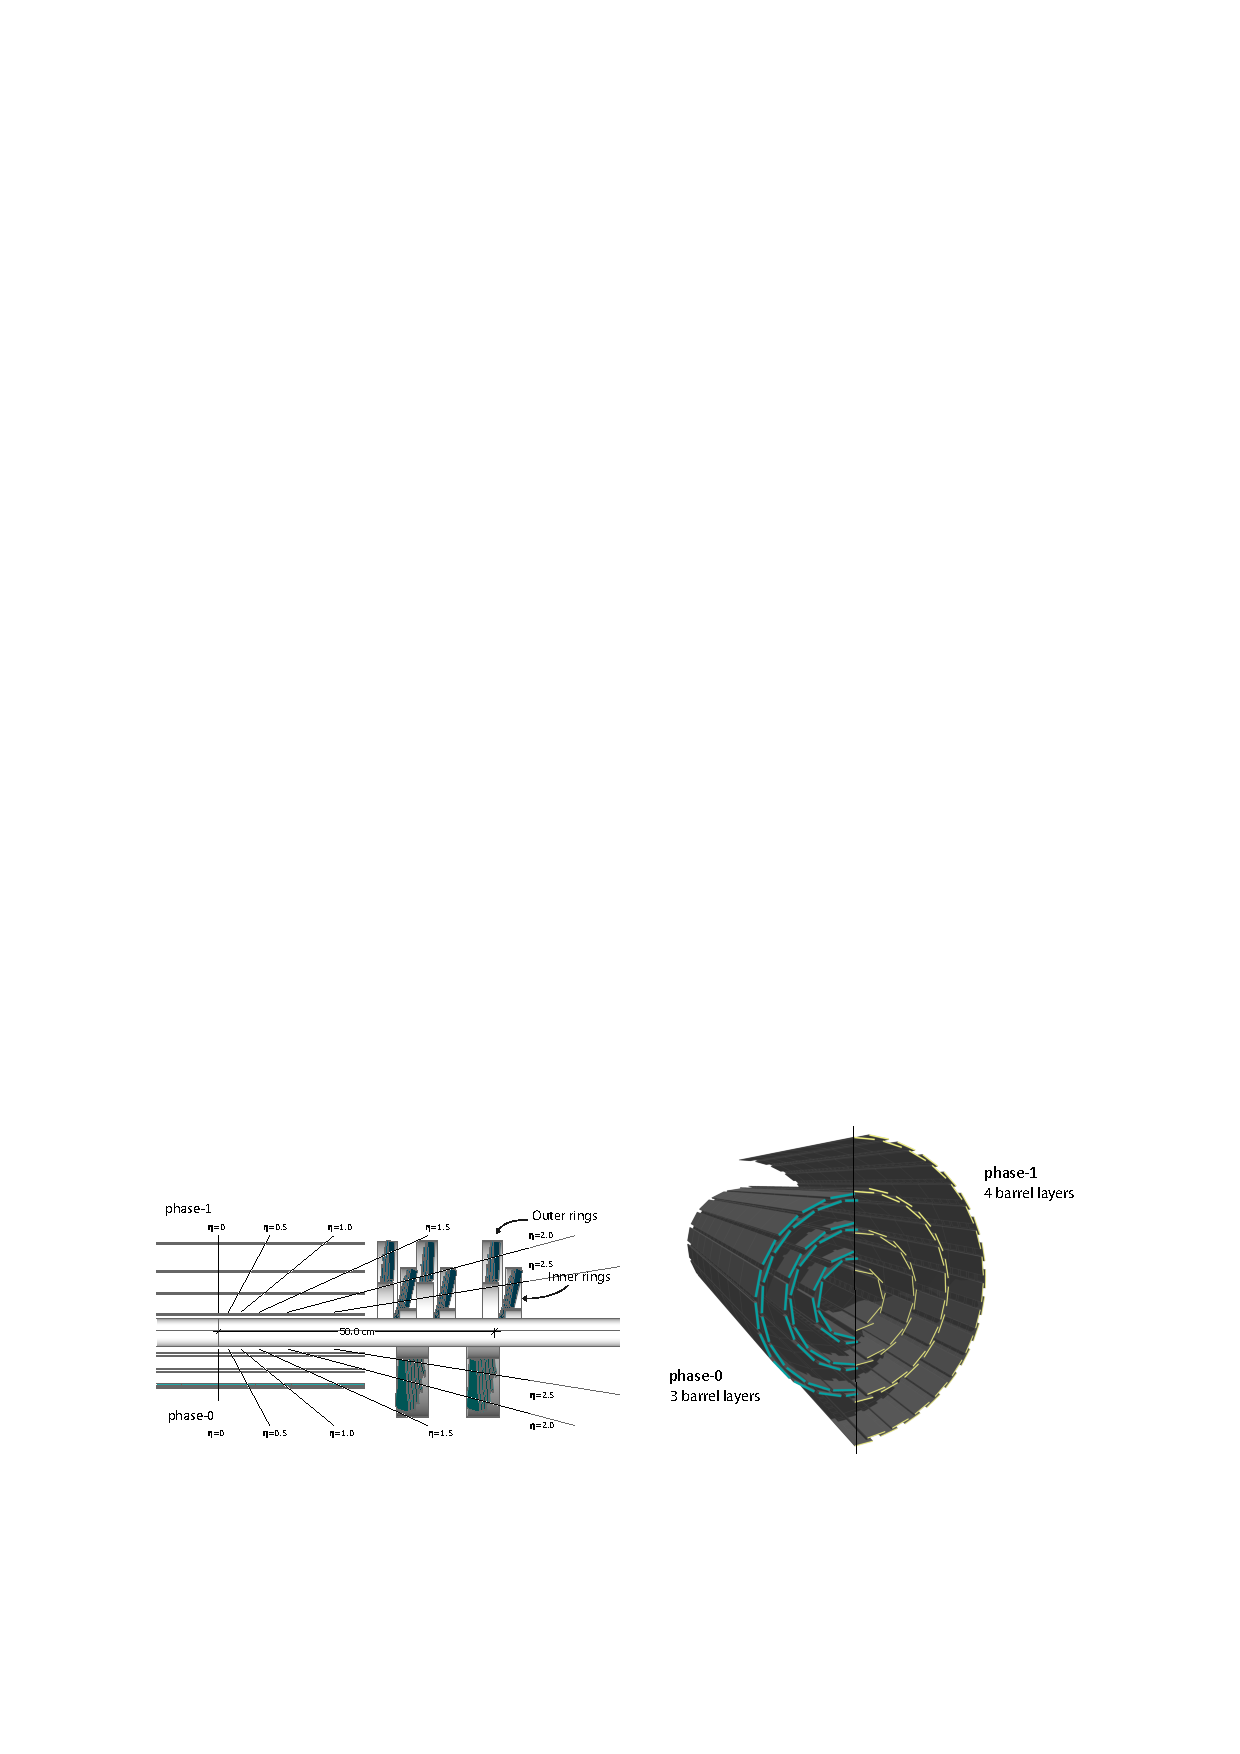
\includegraphics[width=0.98\textwidth]{Immagini/PXLph0ph1.pdf}
\caption{Rappresentazione schematica della geometria delle due versioni del rivelatore a pixel di CMS nella vista $Rz$ e in una vista prospettica della parte barrel.}
\label{fig:PXLph0ph1}
\end{figure}

\end{description}

%\hline
%\hline
%\hline

Lo scopo è ricostruire , con la maggior precisione possibile, le traiettorie delle particelle cariche, identificando vertici primari e secondari. La composizione interna del tracciatore è mostrata in figura \ref{CMStracker}. Il raggio esterno è circa 110 cm e la lunghezza totale circa 540 cm.

Le particelle cariche cedono energia al materiale di cui `e composto il rivelatore inte- ragendo elettromagneticamente con quest’ultimo; l’energia rilasciata forma coppie elettrone lacuna nel semiconduttore che porta a una ionizzazione del materiale e quindi a un rilascio di cariche che opportunamente raccolte permettono di ricavare informazioni sulla posizione della particella.


Nella zona centrale (barrel) e più interna vi è il rivelatore di vertice a pixel, con tre strati distanti 4, 7 e 11 cm dall'asse dei fasci. La dimensione dei pixel è $100x150$ $\mu m^2$. Più esternamente ci sono rivelatori a microstrip tra 20 e 110 cm. Le parti laterali, dette endcap, sono invece costituite da 2 piani a pixel e 9 a microstrip. La parte di microstrip è divisa in due parti Inner Barrel e Outer Barrel, figura \ref{CMStracker}:
\begin{itemize}
\item Tracker Inner Barrel (TIB), costituito di 4 cilindri posti intorno ai piani a pixel.
\item Tracker Inner Discs (TID), 3 dischi posti nella parte interna di endcup.
\item Tracker Outer Barrel (TOB), 6 cilindri che formano la parte esterna del barrel.
\item Tracker EndCaps (TEC), 9 dischi che completano la parte più esterna di endcup.
\end{itemize}

%The Tracker will suffer significant radiation damage by LS3 and must be completely re-
%placed for Phase-II. To maintain adequate track reconstruction performance at the much higher
%PU pileup levels of the HL-LHC, the granularity of both the outer tracker and the pixel systems will
%be increased by roughly a factor 4. In the outer tracker, this will be achieved by shortening the
%lengths of silicon sensor strips relative to those in the current detector, without changing the
%pitch very significantly. A number of design improvements will lead to a much lighter Outer
%Tracker providing significantly improved p T resolution and a lower rate of γ-conversions com-
%pared to the present detector. In addition, the module design will be capable of providing track-stub information to the L1 trigger at 40 MHz for tracks with p T ≥ 2 GeV . This will en-
%sure powerful background rejection at the earliest stage of the event selection. The pixel system
%will implement smaller pixels and thinner sensors for improved impact parameter resolution
%and better two-track separation. This will improve b-tagging as well as τ-hadronic decay and
%track reconstruction efficiencies within boosted jets. With up to 10 additional pixel disks in
%each of the forward regions the system coverage will be extended to close to | η | = 4, to better
%match the range of coverage of the calorimetry.
\subsection{Tracciatore di fase II}

Al fine di mantenere o migliorare le prestazioni di CMS nelle condizioni di alto pile-up e alto danneggiamento da radiazioni, nella fase  di HL-LHC, l'intero sistema di tracciatura delle particelle dovrà essere sostituito con nuovi rivelatori capaci di sostenere livelli di radiazione maggiori e con maggiori funzionalità.
\begin{figure}
\centering
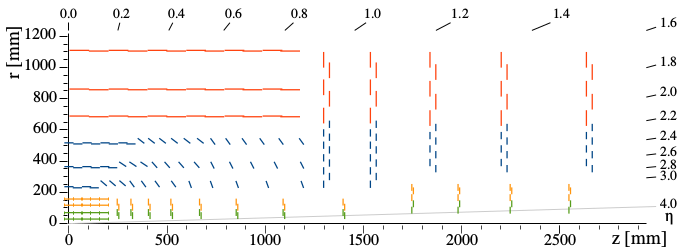
\includegraphics[scale=0.4]{Immagini/TrackerPhaseII}
\caption{Schema rappresentante un quarto del tracciatore. La parte esterna del tracciatore è in blu (moduli PS) e rosso (moduli 2S). La parte del tracciatore a pixel, con l'estensione in avanti è rappresentata in verde e giallo.}
\label{TrackerPhaseII}
\end{figure}

Le limitazioni dell'attuale tracciatore ne impediscono l'utilizzo nella fase di alta luminosità. I principali requisiti per il nuovo rivelatore sono i seguenti, figura \ref{TrackerPhaseII}:

\begin{itemize}
\item \textbf{Tolleranza alla radiazione}: Si prevede che il nuovo tracciatore dovrà operare, mantenendo alta l'efficienza, fino ad una luminosità integrata di 3000 $\mathrm{fb^{-1}}$. Inoltre per la parte esterna del tracciatore non si prevedono interventi di manutenzione, mentre per la parte di tracciatore a pixel sono sotto studio opzioni che consentano di operare sostituzioni nella zona più interna. 
\end{itemize}

\[
\begin{array}{lccc}

\toprule
\mathrm{Regione} & \mathrm{Fluenza \quad massima} [n_{eq}/cm^2] & r [mm] & z[mm]  \\

\midrule

\mathrm{IT \quad barrel \quad layer 1} & 2.3\times10^{16} & 28 & 0\\

\mathrm{IT\quad barrel\quad layer 2} & 5.0\times10^{15} & 69 & 0\\

\mathrm{IT\quad barrel\quad layer 4} & 1.5\times10^{15} & 156 & 89\\

\mathrm{IT\quad forward,\quad ring 1} & 1.0\times10^{16} & 51 & 252\\

\mathrm{IT\quad service\quad cylinder} & 9.6\times10^{14} & 170 & 260\\

\bottomrule
\end{array}
\]

\begin{itemize}
\item \textbf{Alta risoluzione e un migliore sistema di separazione delle tracce}: l'attuale tracciatore ha prestazioni peggiori nel tracciare jet di alta energia, a causa della sovrapposizione di più hit nel rivelatore a pixel. Al fine di sfruttare al meglio la maggiore statistica che ci sarà con HL-LHC, è necessario migliorare la capacità nel distinguere due tracce molto vicine. 
Allo stesso modo  per assicurare alta efficienza, nonostante un maggiore pile-up, è necessaria una maggiore densità di canali di lettura. Come riferimento si stima che la media di pile-up per ogni bunch crossing sarà di circa 140, a fronte dei 40 attuali.

\item \textbf{Riduzione di materiale}: un fattore importante che limita l'attuale risoluzione  è la quantità di materiale che le particelle attraversano. Questo è responsabile di perdita di energia e scattering multipli, i quali causano un peggioramento nelle prestazioni dei calorimetri e nella precisione di ricostruzione dell'evento.

\item \textbf{Sistema di riconoscimento delle tracce affidabile e veloce}: maggiore pile-up significa complicazioni nella ricostruzione delle tracce e tempi più lunghi. La velocità nella ricostruzione è essenziale per la funzionalità del trigger di alto livello (High -Level Trigger). 

\item \textbf{Compatibilità con il nuovo trigger L1}: La selezione degli eventi nella nuova fase ad alta luminosità è una sfida importante, non solo per l'alto numero di particele e quindi tracce, ma anche perché l'alto numero di pile-up rende inefficienti gli algoritmi di selezione degli eventi. Per questo motivo parte del processo di ricostruzione, che attualmente è svolto ad alto livello, sarà spostato in L1il cui rate massimo raggiungerà i 750 kHz.

\item \textbf{Estensione della regione di accettanza delle tracce}: altri benefici per CMS possono essere ottenuti ampliando la copertura della regione in avanti da parte del tracciatore e dei calorimetri.

 
\end{itemize}


\subsection{Tracciatore interno}
La parte interna del tracciatore sarà dotata di moduli a pixel. Come già evidenziato, nella fase ad alta luminosità il punto cruciale per la progettazione sarà la tolleranza alla radiazione di di sensori e elettronica di lettura, come anche la parte di gestione dei dati e l'aumento di frequenza di lavoro per il trigger. 
I candidati per i sensori che  rispettano le richieste su risoluzione, separazione delle tracce e occupazione sono sensori di silicio, di spessore 100-150 $\mu$m, con pixel di 25 $\times$ 100 $\mu m^2$ o 50 $\times$ 50 $\mu m^2$. 
Di conseguenza il chip di lettura dovrà avere celle di piccola dimensione con basse soglie. Lo sviluppo di questo nuovo chip è portato avanti dalla collaborazione RD53 che vede insieme ATLAS e CMS, il progetto prevede un chip con celle di dimensione 2500 $\mu m^2$  in tecnologia CMOS a 65 nm. 
Tale configurazione dovrebbe consentire una migliore resistenza al danneggiamento da radiazione.

\subsubsection{Sensori}
\begin{figure}
\centering
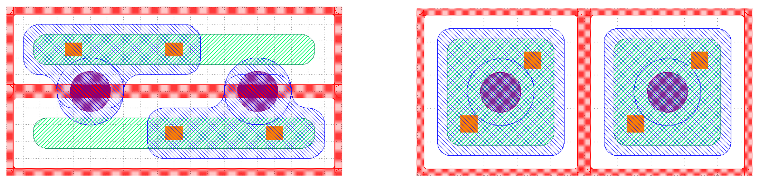
\includegraphics[scale=0.35]{Immagini/Sensors}
\caption{Schema di due celle adiacenti con dimensioni $\mathrm{25 \times 100 \mu m^2}$ (sinistra) e $\mathrm{50 \times 50\mu m^2}$ (destra). Gli impianti n+ sono riportati in verde, in blu le metallizzazioni, in rosso le aree di p-stop , i contatti in arancione e in viola i le piazzole per i bump bond.}
\label{Sensors}
\end{figure}
L'ambiente in cui saranno immersi i sensori nella fase di alta luminosità sarà estremo sia in termini di luminosità integrata che istantanea. 
I sensori saranno esposti ad una fluenza di  $2.3 \times 10^{16} \mathrm{n_{eq}/cm^2}$ negli strati più interni del tracciatore con una luminosità integrata di 3000$\mathrm{fb^{-1}}$. La dose equivalente è circa 12 MGy (1.2 Grad). 
Date queste condizioni si è preferito optare per sensori il più sottili possibile, dato che il vantaggio di raccogliere più carica con sensori più spessi viene annullato dal peggioramento delle prestazioni dovuto all'aumento di difetti nel silicio, a causa dell'alto irraggiamento. 
Lo spessore attivo del sensore, nel caso pixel planare sarà tra i 100 e 150 $\mu$m ( nella fase-0 e fase-1 lo spessore dei pixel era tra i 270  e i 285 $\mu$m). 
Il test di questi sensori insieme ai chip di lettura dimostrerà la fattibilità di utilizzo di questo tipo di sensore in ambienti con alti livelli di radiazione, o se saranno necessarie modifiche. 
Rispetto al tracciatore di CMS di fase-1 l'area dei pixel sarà ridotta di un fattore 6. Le due possibilità prese in considerazione sono $\mathrm{25 \times 100 \mu m^2}$ e  $\mathrm{50 \times 50 \mu m^2}$. 
Nel processo di valutazione dei vari progetti per i pixel particolare rilevanza hanno i seguenti punti:
\begin{itemize}
\item \textbf{Metodo di contro polarizzazione}Schema di polarizzazione dei sensori prima di unirli al chip. Tra le opzioni considerate ci sono l'utilizzo di punch through comuni per polarizzare più pixel contemporaneamente, resistenze in poli-silicio, o l'assenza completa di un metodo di polarizzazione. in assenza di una griglia per la polarizzazione il test dei sensori richiederebbe altre tecniche per aver accesso ai singoli pixel. 

\item \textbf{Isolamento del pixel} isolamento attraverso p-stop o p-spray. Per risparmiare spazio, gli impianti di p-stop sono in comune tra i pixel adiacenti, invece di averne uno per ogni singolo pixel.
\item \textbf{Metal overhangs}
\end{itemize}

CMS ha avviato numerose proposte di $\mathrm{R \& D}$ per sensori planari, al fine di studiare  tutte le possibili opzioni di progetto nei sensori sottili con piccolo pitch. I sensori sono valutati attraverso esperimenti di test beam, prima e dopo irraggiamento, al fine di testare la resistenza alla radiazione, la risoluzione spaziale, l'efficienza di raccolta carica, e non ultima l'efficienza di cella. 
Le proposte includono sia sensori con pixel di dimensione $\mathrm{25 \times 100 \mu m^2}$ che $\mathrm{50 \times 50\mu m^2}$ con vari design . Queste proposte includono sensori compatibili sia con chip di lettura PSI46dig, che con il prototipo di ROC RD53A. 
In figura \ref{Sensors} è mostrato l'aspetto di due celle adiacenti con pixel di dimensione $\mathrm{25 \times 100 \mu m^2}$ (sinistra) e $\mathrm{50 \times 50\mu m^2}$ (destra). Questi sensori sono compatibili con il prototipo RD53A.

\subsubsection{Chip}

\begin{figure}
\centering
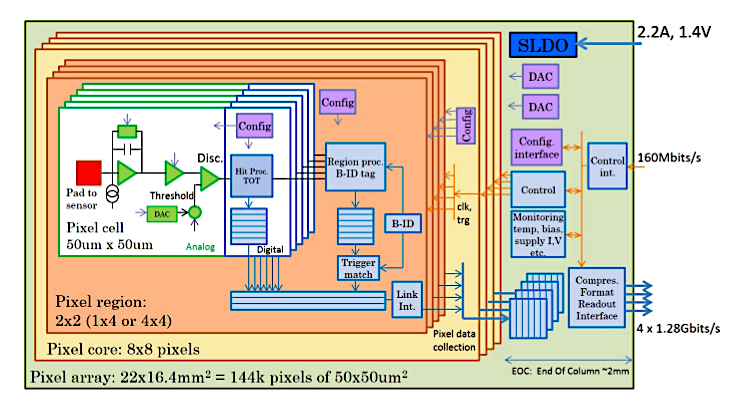
\includegraphics[scale=0.4]{Immagini/ChipBlockDiagram}
\caption{Architettura del chip con bassi livelli di rumore analogico con un sistema di digitalizzazione del ToT a 4 bit. Nello schema sono riportate anche l'interfaccia di controllo, posta nella zona di EOC (End Of Column), l'interfaccia di lettura e il sistema di alimentazione che sfrutta un regolatore di tensione con shunt (Shunt-LDO).}
\label{ChipBlockDiagram}
\end{figure}

La parte cruciale nel sistema di lettura per il tracciatore interno è la progettazione di un chip di lettura dei pixel resistente alle radiazioni. Il diagramma a blocchi del chip è mostrato in figura \ref{ChipBlockDiagram}. 
La carica raccolta su ogni pixel è amplificata, formata e digitalizzata con una risoluzione di 4 bit a 40 MHz, sfruttando l'informazione di ToT (Time Over Threshold)\footnote{Il metodo di ToT consiste nel misurare il tempo durante il quale l'impulso analogico è sopra una certa soglia.}, che viene poi digitalizzata e utilizzata come misura di carica raccolta. 
I segnali vengono memorizzati durante i 12.5 $\mu$s di latenza del trigger\footnote{Si fa riferimento a latenze che si avranno con il trigger di fase II.} e memorizzati localmente in vettori all'interno della regione di pixel (che potrà essere 2 $\times$ 2 o 4 $\times$ 4). 
I dati riguardanti eventi con trigger sono raccolti da questa memoria e dopo un appropriato processo di compressione dati, svolto all'interno del chip, questi sono inviati all'esterno del chip tramite E-links (Electrical links) ad una velocità di 1.28 Gb/s. 
Sempre all'interno del rivelatore sono presenti i moduli di conversione, basati su chip LpGBT, che riversano i dati provenienti da un massimo di 7  E-links in una fibra ottica da 10 Gb/s per il trasporto verso il sistema di acquisizione dati (DAQ), all'esterno del rivelatore. 
I comandi, i dati di configurazione, i segnali di trigger e il clock sono spediti a 2.5 Gb/s verso i moduli di conversione per poi essere convertiti e inviati ai moduli tramite E-links a 160 Mb/s. 
Gli impulsi di calibrazione sono disponibili per tutti i pixel, grazie ad un esteso sistema a doppio impulso che può iniettare due differenti segnali di calibrazione con tempi e livelli programmabili. 
Inoltre è presente la possibilità di monitorare l'attività del chip tramite un 
Sono presenti anche sensori per il controllo della temperatura del chip distribuiti in più punti, in particolare sensori di temperatura sono integrati nella parte del chip che si occupa dell'alimentazione. Questo infatti è il punto con la più alta densità di potenza dissipata, che può variare significativamente in funzione delle configurazioni. 
%All power supply voltages (before and
%after the power regulator) and currents can be measured. In addition, a large number of ana-
%logue operation parameters can be monitored: bias currents for analogue front-ends, band gap
%references, calibration pulse voltages, PLL control voltage, etc. Dedicated features to monitor
%radiation degradation at both single transistor level and digital level (ring oscillators) are also
%included.
Un rapido elenco delle caratteristiche del chip di lettura sono riportate in tabella:

\[
\begin{array}{ll}

\toprule

\midrule

\mathrm{Technology} & \quad 65 \mathrm{nm \quad CMOS}\\

\mathrm{Chip \quad size} & \quad \mathrm{22 mm \times (16.4 mm + 2 mm)} \\

\mathrm{Pixel \quad size} & \quad \mathrm{50 \times 50 \mu m^2, 25 \times 100 \mu m^2)} \\

\mathrm{Number\quad of\quad pixels} & \quad \mathrm{144320} \\

\mathrm{Hit \quad rate} & \quad \mathrm{< 3 GHz/cm^2} \\

\mathrm{Charge \quad resolution} & \quad \mathrm{24 bit \quad ToT} \\


\bottomrule
\end{array}
\]

%si può allungare la lista

Le richieste tecniche per questo nuovo PROC (Pixel Read Out Chip) hanno portato ad l'utilizzo di moderna tecnologia CMOS a consumi ridotti ed alta densità con alimentazione a bassa tensione, circa 1.2 V. Questo fa si che il chip sia alimentato con correnti significative, circa 2.2 A per chip. 
La prima idea potrebbe essere quella di utilizzare convertitori DC-DC locali, ma questa possibilità è esclusa  a causa dell'ambiente ricco di radiazioni, del poco spazio disponibile e del tentativo di limitare il più possibile la quantità di materiale nel tracciatore. 

\begin{figure}
\centering
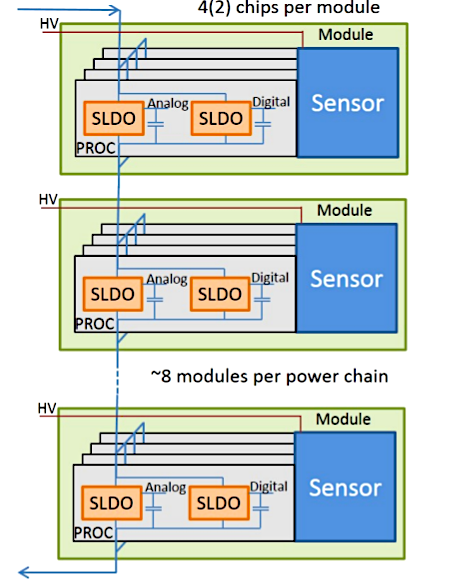
\includegraphics[scale=0.4]{Immagini/serial}
\caption{Sistema di alimentazione seriale dei moduli, ognuno dei quali ha al suo interno 4 o 2 chip in parallelo. Sul chip l'alimentazione è gestita da due SLDO in parallelo, uno per la parte digitale e uno per quella analogica.}
\label{serial}
\end{figure}

La soluzione scelta è dunque quella di utilizzare un sistema di alimentazione seriale, ciò permetto l'utilizzo di un quantitativo minimo di materiale e mantiene a livelli accettabili la perdita di potenza sui cavi. 
La catena è composta da 8-10 moduli ognuno con 2 o 4 chip connessi in parallelo, come si può vedere in figura \ref{serial}. 
All'interno del chip è incluso circuito ottimizzato per l'alimentazione che combina le capacità di uno shunt di corrente e di un regolatore LDO (Low DropOut), chiamato Shunt-LDO (SLDO). 
Come vedremo nel capitolo successivo lo SLDO assicura un consumo di corrente/potenza costante, indipendentemente dal rate di eventi e di trigger. 
Inoltre grazie ad una attenta progettazione è assicurata una suddivisione delle correnti appropriata tra i vari chip posti in parallelo all'interno del modulo. Lo stesso chip al suo interno ha due SLDO in parallelo uno per la parte analogica e uno per quella digitale. 
Questa separazione è resa necessaria per rendere minima l'influenza del rumore della parte digitale su la parte analogica, più sensibile  al rumore.